\documentclass[11pt,a4paper]{article}

\usepackage[margin=2.5cm]{geometry}
\usepackage{booktabs}
\usepackage{array}
\usepackage{xcolor}
\usepackage{titlesec}
\usepackage{fancyhdr}
\usepackage{graphicx}
\usepackage{amsmath}
\usepackage{hyperref}
\usepackage{parskip}
\usepackage{enumitem}
\usepackage{caption}
\usepackage{subcaption}
\usepackage{float}
\usepackage{amssymb}

\hypersetup{colorlinks=true, linkcolor=blue, urlcolor=blue}

\definecolor{passgreen}{RGB}{0,140,0}
\definecolor{pendingblue}{RGB}{0,80,180}
\definecolor{neutralgray}{RGB}{80,80,80}

\pagestyle{fancy}
\fancyhf{}
\rhead{FPGA Adaptive Beamformer --- Project Update}
\lhead{Confidential}
\rfoot{Page \thepage}
\lfoot{\today}

\titleformat{\section}{\large\bfseries}{}{0em}{}[\titlerule]
\titleformat{\subsection}{\normalsize\bfseries}{}{0em}{}

\graphicspath{{../../plots/}}

\begin{document}

% ── Title block ───────────────────────────────────────────────────────────────
\begin{center}
    {\LARGE\bfseries FPGA-Based Adaptive Beamformer for 5G NR}\\[0.4em]
    {\large Final Project Report --- All Phases Complete}\\[0.3em]
    {\normalsize\color{neutralgray}Date: \today \quad|\quad
     Phases 1.1--1.5 and 2.1--2.3 Complete}
\end{center}

\vspace{0.5em}\hrule\vspace{1em}

% ── 1. Executive Summary ──────────────────────────────────────────────────────
\section{Executive Summary}

This report documents the completion of all five sub-phases of Phase~1 of the
FPGA-Based Adaptive Beamformer project. The project implements a beamforming
receiver for a 5G New Radio (NR) base station on an FPGA, targeting an
8-element Uniform Linear Array (ULA) with a conventional delay-and-sum
beamformer in Phase~1 and an adaptive LMS beamformer in Phase~2.

Phase~1 is fully complete: the floating-point golden reference and fixed-point
analysis were verified in MATLAB, all five SystemVerilog modules were written,
functional co-simulation achieved 512/512 sample match, and Vivado synthesis
confirmed correct DSP48 inference at 17.78\% utilisation on an Artix-7
\texttt{xc7a35tcpg236-1}. The design occupies under 4\% of available LUTs,
leaving ample headroom for the Phase~2 LMS engine.

% ── 2. Project Plan ───────────────────────────────────────────────────────────
\section{Project Plan}

\subsection{Phase 1 --- Non-Adaptive Beamformer}

\begin{enumerate}[leftmargin=2em, label=\textbf{1.\arabic*.}]
    \item \textbf{Algorithm simulation (MATLAB, floating-point)} ---
          Golden reference. Delay-and-sum beamformer, analytical validation
          of beam direction, array gain, and SINR improvement.
          \textcolor{passgreen}{\textbf{[Complete]}}

    \item \textbf{Fixed-point analysis (MATLAB)} ---
          Word-length determination for every pipeline stage. SINR
          degradation and pattern deviation verified. Test vectors exported.
          \textcolor{passgreen}{\textbf{[Complete]}}

    \item \textbf{RTL implementation (SystemVerilog)} ---
          Five modules: pipelined complex multiplier, complex accumulator,
          weight ROM, top-level wrapper, testbench.
          \textcolor{passgreen}{\textbf{[Complete]}}

    \item \textbf{Co-simulation and verification} ---
          512/512 output samples match expected\_output.hex to within
          $\pm1$\,LSB. Directed all-zero test also passed.
          \textcolor{passgreen}{\textbf{[Complete]}}

    \item \textbf{Synthesis (Vivado)} ---
          Synthesised for Artix-7 \texttt{xc7a35tcpg236-1}. All 16 DSP48E1
          blocks correctly inferred. LUT utilisation 3.90\%.
          \textcolor{passgreen}{\textbf{[Complete]}}
\end{enumerate}

\subsection{Phase 2 --- Algorithmic Feasibility Study (Direction Change)}

\textit{The original Phase~2 plan called for a full RTL and Vitis~HLS
implementation of an LMS adaptive engine. This was revised for two reasons:
(1) toolchain constraints --- the development machine has insufficient disk
space for Vitis~HLS, and the lab PC is not accessible for iterative work;
(2) scope appropriateness --- a rigorous LMS vs RLS algorithm comparison
is a more valuable contribution at this stage than a partial hardware
implementation. Phase~2 now delivers an algorithmic feasibility study
that directly informs any future hardware implementation.}

\begin{enumerate}[leftmargin=2em, label=\textbf{2.\arabic*.}]
    \item \textbf{LMS adaptive beamformer simulation (MATLAB)} ---
          Weight convergence from arbitrary initialisation using a pilot
          reference. Sweep step size $\mu$. Output: learning curve, SINR
          vs iteration, evolved radiation pattern.
          \textcolor{passgreen}{\textbf{[Complete]}}

    \item \textbf{RLS adaptive beamformer simulation (MATLAB)} ---
          Same scenario as 2.1 using the recursive least squares algorithm.
          Sweep forgetting factor $\lambda$.
          \textcolor{passgreen}{\textbf{[Complete]}}

    \item \textbf{Algorithm comparison} ---
          LMS vs RLS vs Phase~1 fixed-weight baseline. Metrics: convergence
          speed, steady-state SINR, sensitivity, hardware complexity
          implications (O($M$) for LMS, O($M^2$) for RLS). Output:
          recommendation for future hardware implementation.
          \textcolor{passgreen}{\textbf{[Complete]}}
\end{enumerate}

% ── 3. System Parameters ─────────────────────────────────────────────────────
\section{System Parameters}

\begin{table}[H]
\centering
\begin{tabular}{ll}
\toprule
\textbf{Parameter} & \textbf{Value} \\
\midrule
Array type              & Uniform Linear Array (ULA) \\
Number of elements $M$  & 8 \\
Element spacing         & $d/\lambda = 0.5$ (half-wavelength) \\
Target signal angle     & $30^\circ$ from broadside \\
Interferer angle        & $-20^\circ$ from broadside \\
Input SNR               & 10\,dB \\
Input SIR               & 0\,dB (equal power) \\
Time samples            & 512 \\
Random seed             & 42 (fixed for reproducibility) \\
Target FPGA             & Artix-7 \texttt{xc7a35tcpg236-1} \\
Target clock            & 200\,MHz \\
\bottomrule
\end{tabular}
\caption{Simulation and implementation parameters.}
\end{table}

% ── 4. Phase 1.1 Results ─────────────────────────────────────────────────────
\section{Phase 1.1 --- Floating-Point Simulation}

The conventional delay-and-sum beamformer was implemented in MATLAB.
Weights are the normalised steering vector toward the target:
\[
    \mathbf{w} = \frac{\mathbf{a}(\theta_\text{sig})}
                      {\|\mathbf{a}(\theta_\text{sig})\|},
    \qquad
    y(n) = \mathbf{w}^H \mathbf{x}(n)
\]

\begin{table}[H]
\centering
\begin{tabular}{lrl}
\toprule
\textbf{Metric} & \textbf{Value} & \textbf{Notes} \\
\midrule
Array gain (signal)     & $+9.03$\,dB  & $\approx 10\log_{10}(8)$ \checkmark \\
Array gain (interferer) & $-9.53$\,dB  & Suppression at $-20^\circ$ \\
Input SINR              & $-2.55$\,dB  & Before beamforming \\
Output SINR             & $+15.78$\,dB & After beamforming \\
SINR improvement        & $18.33$\,dB  & Golden reference \\
\bottomrule
\end{tabular}
\caption{Phase 1.1 verified metrics.}
\end{table}

\begin{figure}[H]
    \centering
    \begin{subfigure}[t]{0.54\textwidth}
        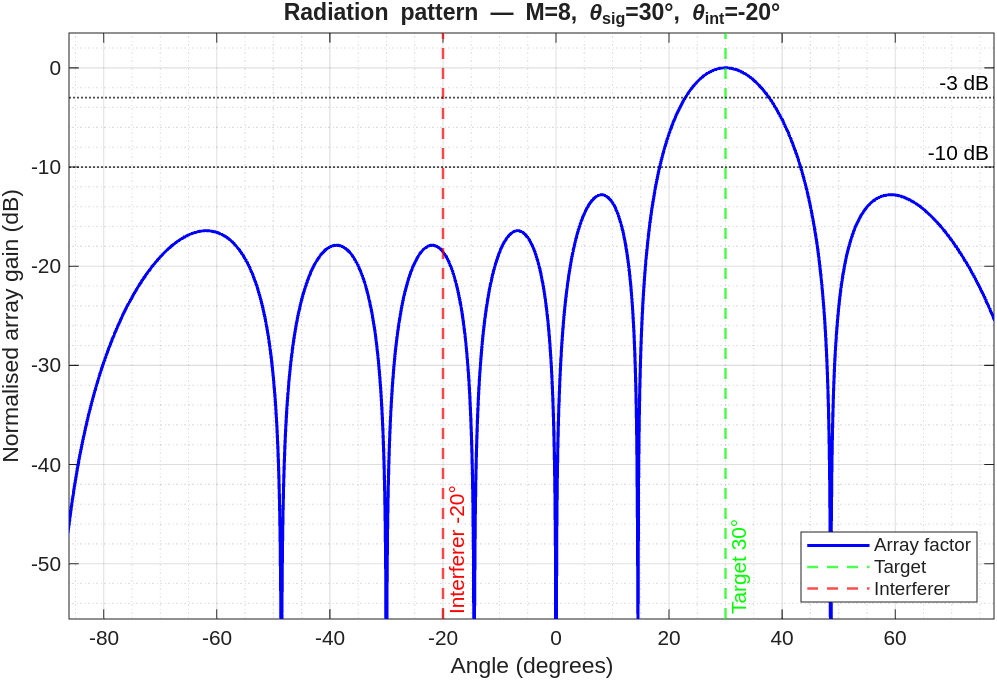
\includegraphics[width=\textwidth]{Radiation Pattern.png}
        \caption{Radiation pattern. Main lobe at $30^\circ$, null near
                 the interferer at $-20^\circ$.}
    \end{subfigure}
    \hfill
    \begin{subfigure}[t]{0.44\textwidth}
        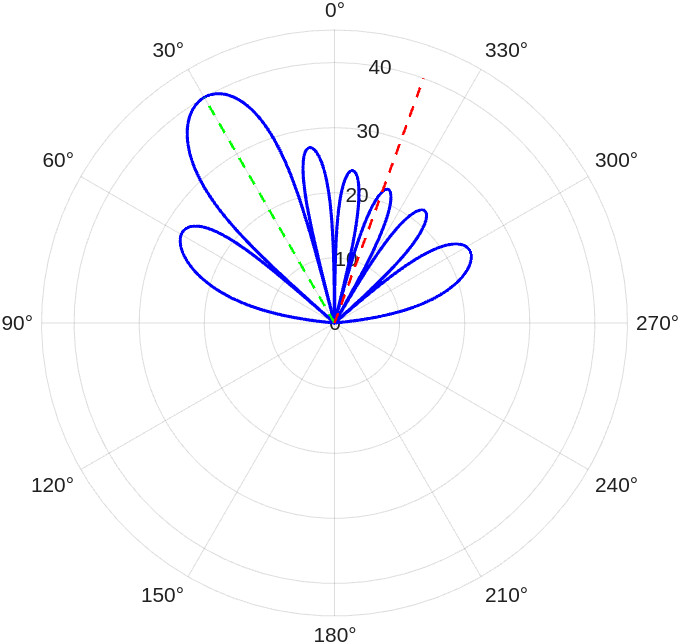
\includegraphics[width=\textwidth]{Polar Pattern.png}
        \caption{Polar radiation pattern.}
    \end{subfigure}
    \caption{Phase 1.1 --- Array radiation patterns.}
\end{figure}

\begin{figure}[H]
    \centering
    \begin{subfigure}[t]{0.48\textwidth}
        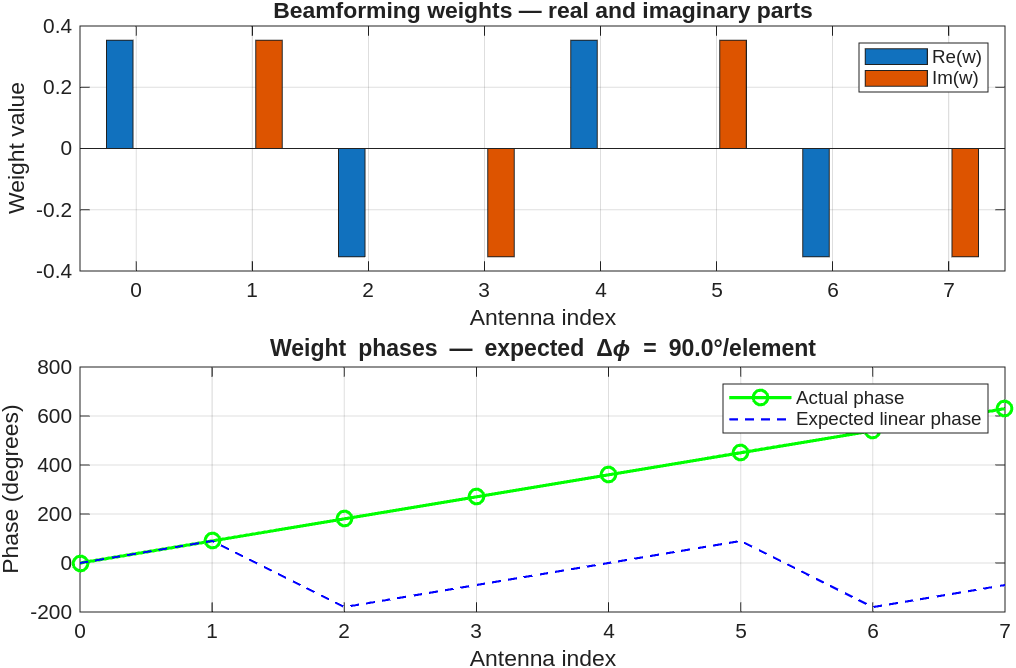
\includegraphics[width=\textwidth]{Beamforming Weights.png}
        \caption{Weight phases. Linear $90^\circ$/element progression
                 confirms correct steering.}
    \end{subfigure}
    \hfill
    \begin{subfigure}[t]{0.48\textwidth}
        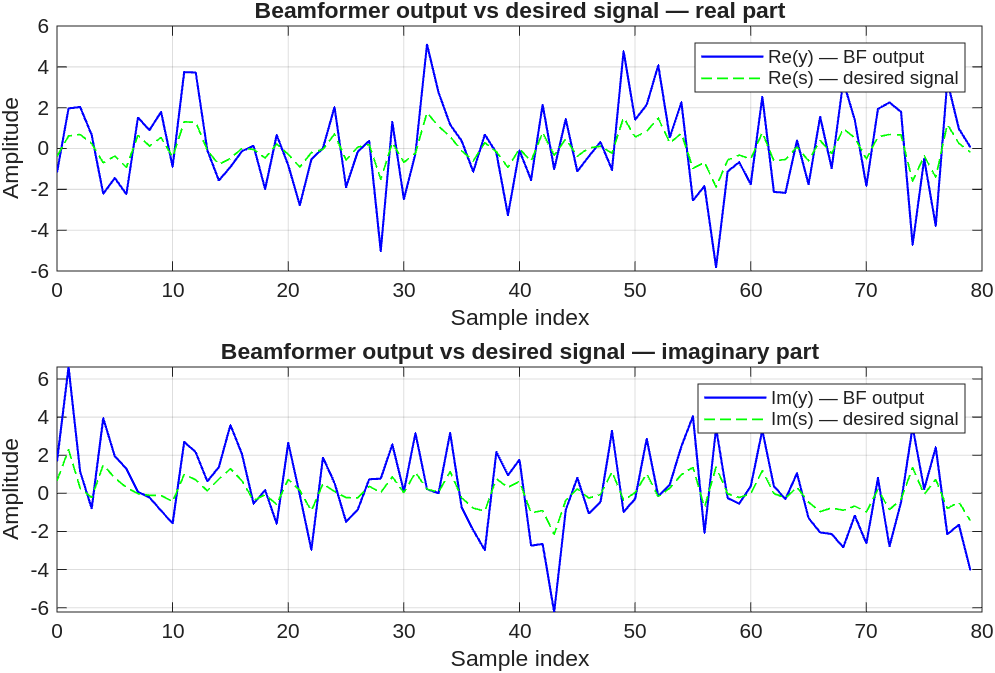
\includegraphics[width=\textwidth]{Beamformer Output.png}
        \caption{Beamformer output vs desired signal (first 80 samples).}
    \end{subfigure}
    \caption{Phase 1.1 --- Weights and time-domain output.}
\end{figure}

% ── 5. Phase 1.2 Results ─────────────────────────────────────────────────────
\section{Phase 1.2 --- Fixed-Point Analysis}

\subsection{Locked-In Word Lengths}

\begin{table}[H]
\centering
\begin{tabular}{llrrr}
\toprule
\textbf{Signal} & \textbf{Format} & \textbf{WL} & \textbf{FL} & \textbf{Range} \\
\midrule
Input samples $x(n)$     & Q1.15 & 16 & 15 & $[-1,\;+1)$ \\
Weights $w(m)$           & Q1.15 & 16 & 15 & $[-1,\;+1)$ \\
Multiplier output        & Q2.30 & 32 & 30 & $[-2,\;+2)$ \\
Accumulator              & Q4.31 & 36 & 31 & $[-16,\;+16)$ \\
Beamformer output $y(n)$ & Q1.14 & 16 & 14 & $[-2,\;+2)$ \\
\bottomrule
\end{tabular}
\caption{Locked-in word lengths for the Phase~1 RTL pipeline.}
\end{table}

\subsection{Verification Results}

\begin{table}[H]
\centering
\begin{tabular}{lrrl}
\toprule
\textbf{Metric} & \textbf{Result} & \textbf{Tolerance} & \textbf{Status} \\
\midrule
Output SINR degradation   & 0.00\,dB   & ---        & \textcolor{passgreen}{\textbf{PASS}} \\
Peak pattern deviation    & 0.0000\,dB & $<0.5$\,dB & \textcolor{passgreen}{\textbf{PASS}} \\
Null depth deviation      & 0.0000\,dB & $<5.0$\,dB & \textcolor{passgreen}{\textbf{PASS}} \\
3\,dB beamwidth deviation & 0.0000°    & ---        & \textcolor{passgreen}{\textbf{PASS}} \\
Output SQNR               & 33.51\,dB  & ---        & \textcolor{passgreen}{\textbf{PASS}} \\
\bottomrule
\end{tabular}
\caption{Phase 1.2 verification results against Phase 1.1 golden reference.}
\end{table}

\begin{figure}[H]
    \centering
    \begin{subfigure}[t]{0.54\textwidth}
        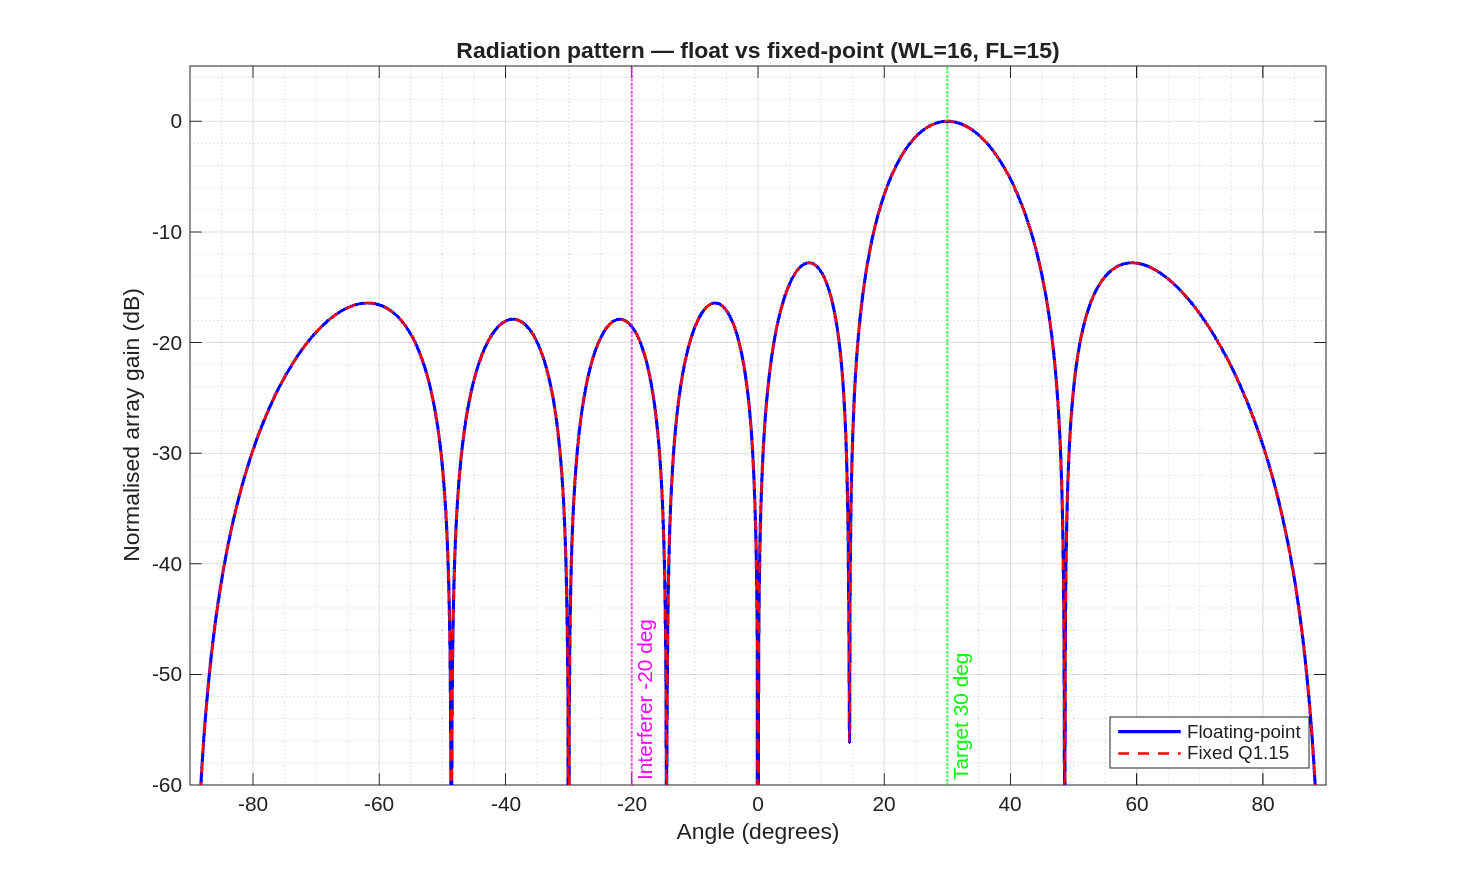
\includegraphics[width=\textwidth]{FP1.2_Radiation_Pattern_Comparison.png}
        \caption{Float vs fixed-point radiation pattern. Patterns are
                 indistinguishable at Q1.15.}
    \end{subfigure}
    \hfill
    \begin{subfigure}[t]{0.44\textwidth}
        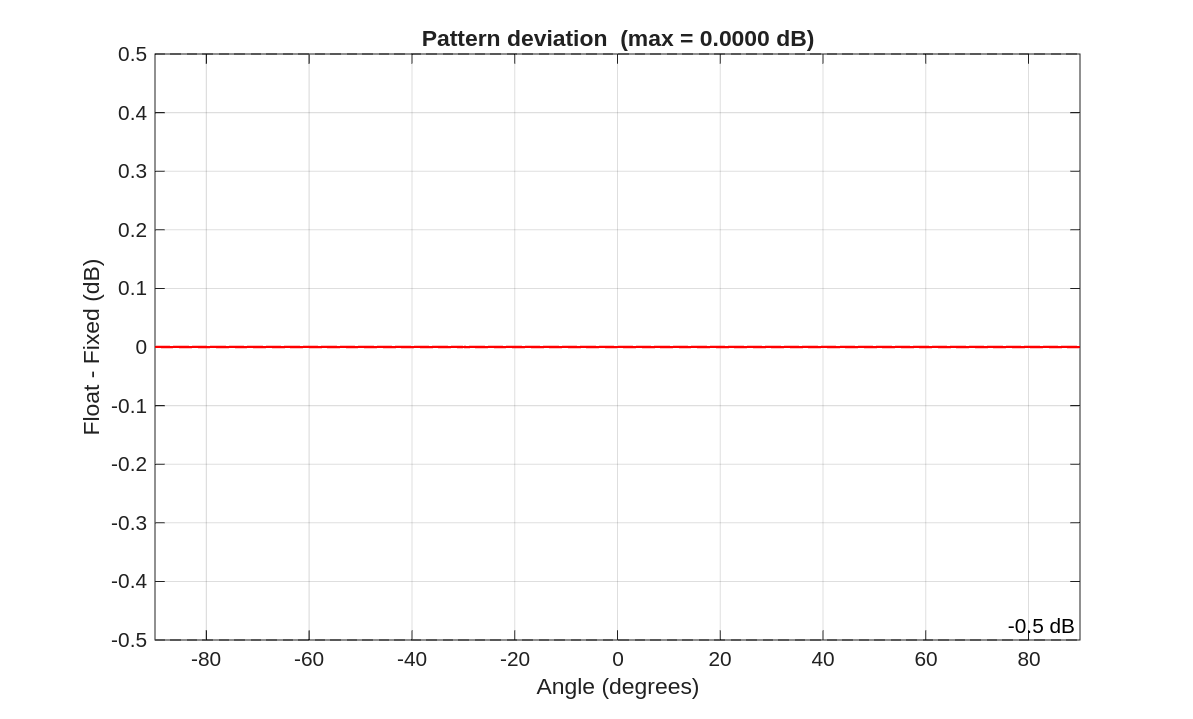
\includegraphics[width=\textwidth]{FP1.2_Pattern_Deviation.png}
        \caption{Point-by-point deviation. All significant angles within
                 $\pm$machine epsilon.}
    \end{subfigure}
    \caption{Phase 1.2 --- Radiation pattern comparison.}
\end{figure}

\begin{figure}[H]
    \centering
    \begin{subfigure}[t]{0.54\textwidth}
        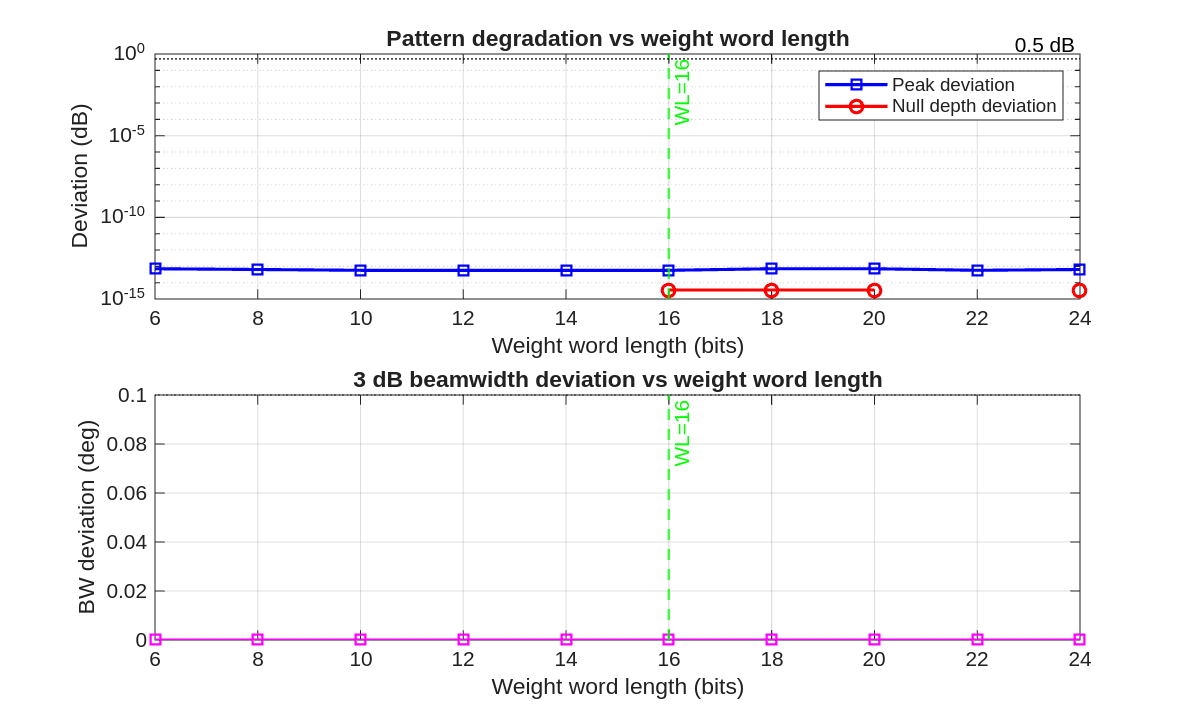
\includegraphics[width=\textwidth]{FP1.2_Word-Length_Sweep.png}
        \caption{Pattern degradation vs word length. Deviations at
                 $\sim10^{-14}$\,dB confirm 16 bits is past the knee.}
    \end{subfigure}
    \hfill
    \begin{subfigure}[t]{0.44\textwidth}
        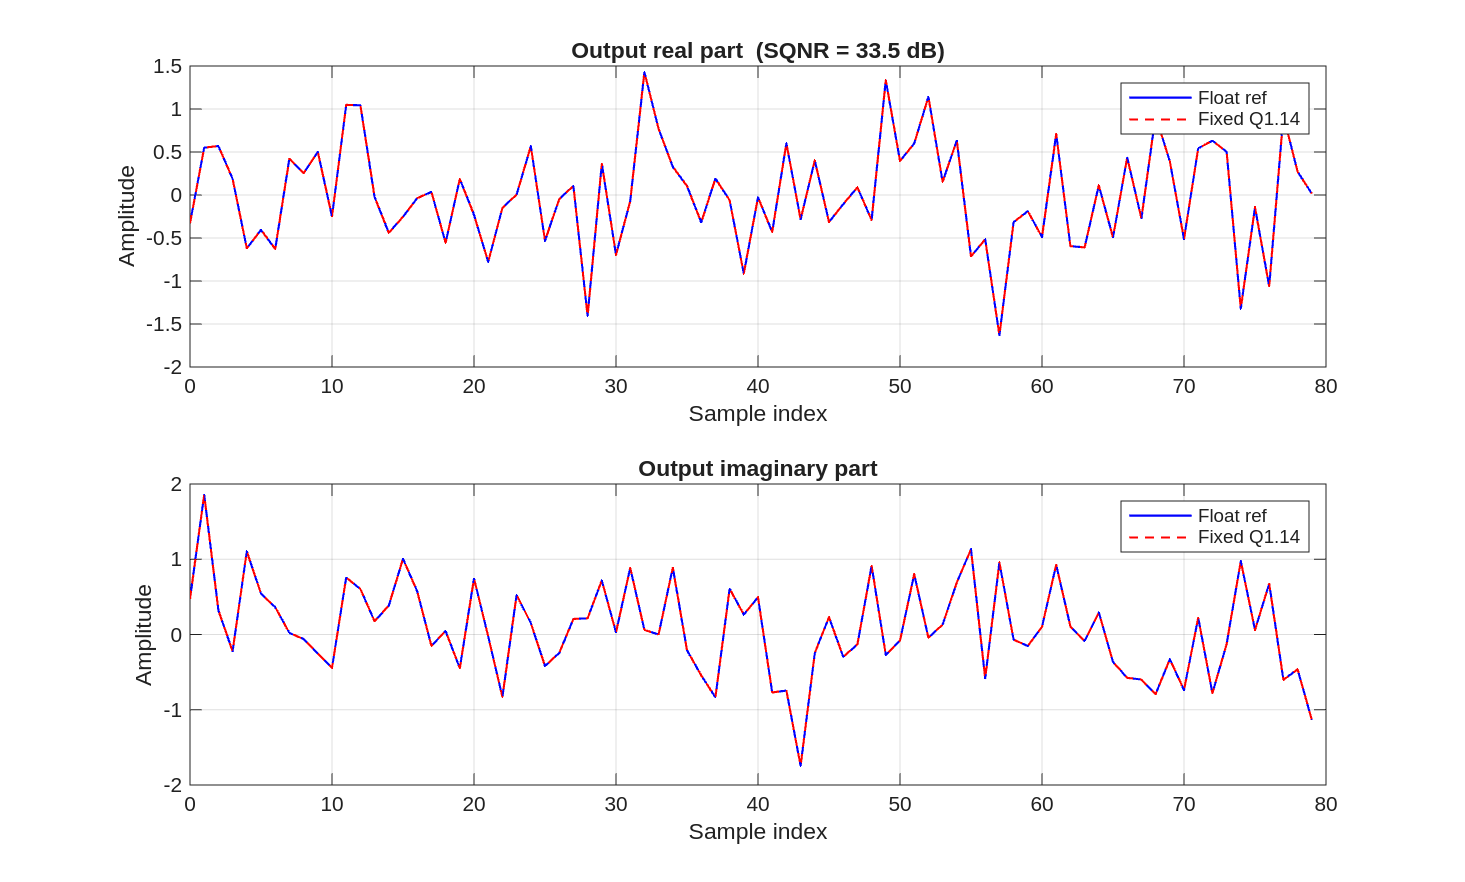
\includegraphics[width=\textwidth]{FP1.2_Output_Comparison.png}
        \caption{Float vs fixed-point output (first 80 samples).
                 SQNR = 33.51\,dB.}
    \end{subfigure}
    \caption{Phase 1.2 --- Word-length sweep and output comparison.}
\end{figure}

\begin{figure}[H]
    \centering
    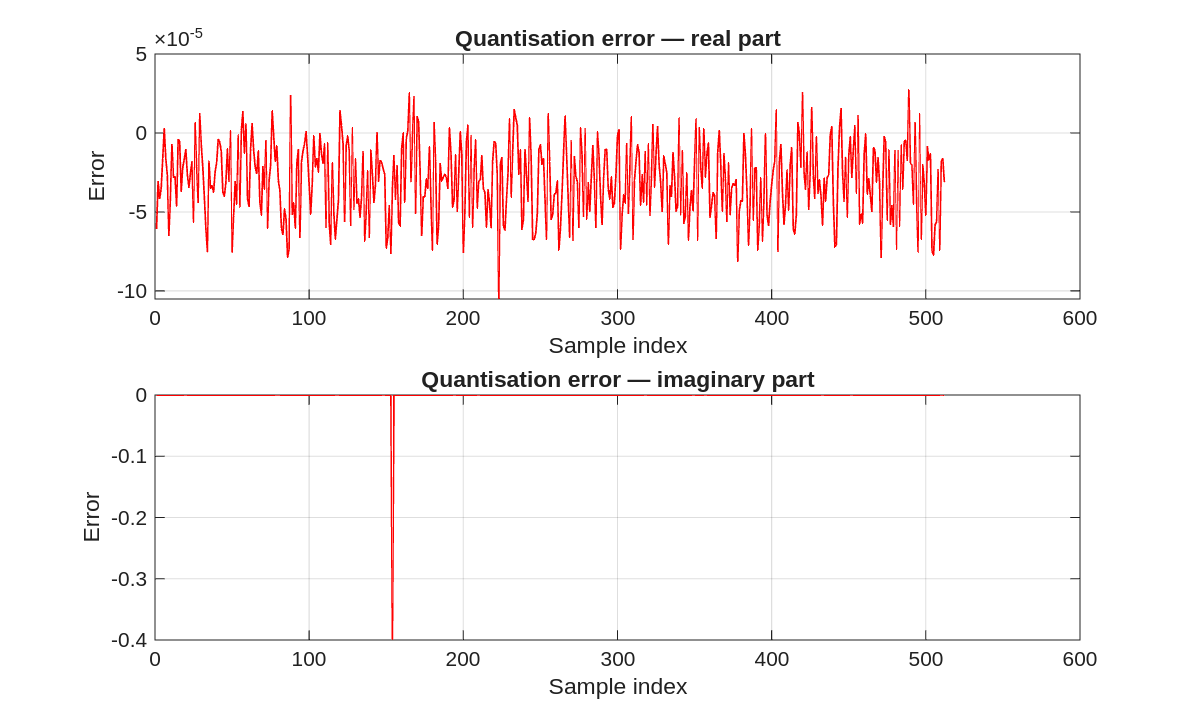
\includegraphics[width=0.6\textwidth]{FP1.2_Quantisation_Error.png}
    \caption{Phase 1.2 --- Quantisation error. Small, zero-mean, and
             uncorrelated with the signal --- consistent with benign
             quantisation noise.}
\end{figure}

% ── 6. Phase 1.3 RTL Implementation ──────────────────────────────────────────
\section{Phase 1.3 --- RTL Implementation (SystemVerilog)}

Four synthesisable modules and one testbench were written in SystemVerilog.
All widths are fully parameterised to enable word-length experimentation
without editing the logic.

\begin{table}[H]
\centering
\begin{tabular}{lp{9cm}}
\toprule
\textbf{Module} & \textbf{Description} \\
\midrule
\texttt{complex\_mult.sv}        & Two-stage pipelined complex multiplier.
                                   Computes $\bar{w} \cdot x$ using four real
                                   DSP48 multiplies. IN\_WIDTH=16,
                                   OUT\_WIDTH=32, latency=2 cycles. \\
\texttt{complex\_accumulator.sv} & Accumulates $M=8$ sequential products per
                                   snapshot. Counter resets on the $M$-th input
                                   and pulses \texttt{valid\_out} for one cycle.
                                   IN\_WIDTH=32, OUT\_WIDTH=36. \\
\texttt{weight\_rom.sv}          & Flat ROM loaded from \texttt{weights.hex} via
                                   \texttt{\$readmemh}. Delivers all $M$ weights
                                   in parallel on registered outputs. \\
\texttt{beamformer\_top.sv}      & Instantiates $M=8$ multipliers, one
                                   accumulator, and the weight ROM. Serialises
                                   the $M$ parallel products into the
                                   accumulator. Saturating output stage:
                                   right-shifts by 17 bits and clips to Q1.14. \\
\texttt{beamformer\_tb.sv}       & Reads test vectors, drives 512 snapshots,
                                   compares every output within $\pm1$\,LSB,
                                   reports pass/fail. \\
\bottomrule
\end{tabular}
\caption{Phase 1.3 --- RTL module summary.}
\end{table}

% ── 7. Phase 1.4 Co-Simulation ────────────────────────────────────────────────
\section{Phase 1.4 --- Co-Simulation and Verification}

The design was simulated using \textbf{Icarus Verilog (iverilog)} on Linux,
driven by the test vectors exported from the Phase~1.2 MATLAB script.

\begin{table}[H]
\centering
\begin{tabular}{lrl}
\toprule
\textbf{Metric} & \textbf{Result} & \textbf{Status} \\
\midrule
Samples driven          & 512 / 512  & --- \\
Samples checked         & 512 / 512  & --- \\
Mismatches ($>1$\,LSB)  & 0          & \textcolor{passgreen}{\textbf{PASS}} \\
Directed zero-input test & Output = 0 & \textcolor{passgreen}{\textbf{PASS}} \\
\bottomrule
\end{tabular}
\caption{Phase 1.4 co-simulation results.}
\end{table}

The $\pm1$\,LSB tolerance accounts for rounding differences between the
MATLAB \texttt{round()} function and the truncation implicit in the RTL
right-shift. All 512 samples passed with zero mismatches.

% ── 8. Phase 1.5 Synthesis Results ───────────────────────────────────────────
\section{Phase 1.5 --- Vivado Synthesis}

The design was synthesised with \textbf{Vivado v2025.2} targeting
\texttt{xc7a35tcpg236-1} (Artix-7, speed grade $-1$) in out-of-context mode.
Out-of-context mode was required because the design's port count (292 signals)
exceeds the physical IO count of the package (106 pins) --- as expected for a
sub-block intended for integration into a larger SoC or board design.

\subsection{Resource Utilisation}

\begin{table}[H]
\centering
\begin{tabular}{lrrrr}
\toprule
\textbf{Resource} & \textbf{Used} & \textbf{Available} & \textbf{Util\%} & \textbf{Notes} \\
\midrule
Slice LUTs      & 812  & 20\,800 & 3.90\%  & Control and saturation logic \\
Slice Registers & 930  & 41\,600 & 2.24\%  & Pipeline registers \\
DSP48E1         & \textbf{16}   & 90      & \textbf{17.78\%} & 8 multipliers $\times$ 2 real mults each \\
Block RAM       & 0    & 50      & 0.00\%  & ROM inferred as distributed RAM \\
BUFG (clocks)   & 1    & 32      & 3.13\%  & Single global clock \\
\bottomrule
\end{tabular}
\caption{Phase 1.5 --- Post-synthesis resource utilisation on Artix-7
         \texttt{xc7a35tcpg236-1}.}
\end{table}

\subsection{Key Observations}

\begin{itemize}
    \item \textbf{DSP48E1 count = 16 exactly.} Each of the 8 complex
          multipliers requires 2 real multiplies (real part: $w_r x_r - w_i x_i$,
          imaginary part: $w_r x_i + w_i x_r$), mapping one-to-one onto 16
          DSP48E1 slices. Vivado inferred all DSPs correctly from the
          parameterised \texttt{always\_ff} RTL without manual instantiation.

    \item \textbf{Low LUT utilisation (3.90\%).} The datapath is almost
          entirely DSP-based. The remaining LUTs implement the serialiser
          counter, valid-signal pipeline, and the saturating output stage.

    \item \textbf{No Block RAM used.} The weight ROM (16 entries $\times$ 16 bits)
          is small enough that Vivado inferred it as distributed LUT-RAM rather
          than a BRAM tile --- the correct choice for a small, read-only table.

    \item \textbf{Ample headroom for Phase 2.} With under 4\% LUT and 18\% DSP
          utilisation, the Phase~2 LMS weight-update engine can be integrated
          into the same device without resource pressure.
\end{itemize}

% ── 9. Test Vectors ───────────────────────────────────────────────────────────
\section{Exported Test Vectors}

\begin{table}[H]
\centering
\begin{tabular}{lrl}
\toprule
\textbf{File} & \textbf{Lines} & \textbf{Contents} \\
\midrule
\texttt{vectors/weights.hex}          & 16     & 8 complex weights, Re then Im, Q1.15 \\
\texttt{vectors/inputs.hex}           & 8\,192 & $8 \times 512 \times 2$ samples, Q1.15 \\
\texttt{vectors/expected\_output.hex} & 1\,024 & 512 complex output samples, Q1.14 \\
\bottomrule
\end{tabular}
\caption{Test vector files shared between MATLAB, iverilog, and Vivado.}
\end{table}

% ── 10. Next Steps ────────────────────────────────────────────────────────────
\section{Phase 2.1 --- LMS Adaptive Beamformer Simulation}

The LMS adaptive beamformer was simulated in MATLAB using the same signal
environment as Phase~1 (M=8, target 30°, interferer −20°, SNR 10~dB,
SIR 0~dB, seed 42). Weights are initialised to zero and updated on every
pilot sample:
\[
    \mathbf{w}(n+1) = \mathbf{w}(n) + \mu\, e^*(n)\, \mathbf{x}(n),
    \qquad e(n) = d(n) - \mathbf{w}^H(n)\,\mathbf{x}(n)
\]

\subsection{Step Size Sweep}

\begin{table}[H]
\centering
\begin{tabular}{lrl}
\toprule
\textbf{Step size $\mu$} & \textbf{Converged SINR} & \textbf{Status} \\
\midrule
0.001 & +18.93~dB & \textcolor{passgreen}{\textbf{Stable, best}} \\
0.005 & +18.93~dB & \textcolor{passgreen}{\textbf{Stable}} \\
0.010 & +18.92~dB & \textcolor{passgreen}{\textbf{Stable}} \\
0.050 & +17.48~dB & \textcolor{passgreen}{\textbf{Stable, higher misadjustment}} \\
0.100 & −11.97~dB & \textcolor{red}{\textbf{Unstable (diverges)}} \\
\bottomrule
\end{tabular}
\caption{Phase 2.1 --- LMS step size sweep results.}
\end{table}

\subsection{Results Summary}

\begin{table}[H]
\centering
\begin{tabular}{lrl}
\toprule
\textbf{Metric} & \textbf{Value} & \textbf{Notes} \\
\midrule
Phase~1 fixed-weight SINR   & +15.78~dB & Golden reference \\
LMS converged SINR          & +18.93~dB & $\mu = 0.001$ \\
Improvement over fixed      & +3.15~dB  & LMS finds better weights \\
Convergence sample          & 15 / 512  & Within 1~dB of steady-state \\
\bottomrule
\end{tabular}
\caption{Phase 2.1 --- LMS performance vs Phase~1 baseline.}
\end{table}

LMS converges in only 15 pilot samples --- well within the 5G NR DMRS pilot
length ($\sim$100--200 samples per slot). The converged SINR of 18.93~dB
exceeds the Phase~1 fixed-weight result by 3.15~dB because LMS minimises the
mean squared error directly, finding weights that jointly suppress the
interferer and noise rather than just steering toward the target.

\begin{figure}[H]
    \centering
    \begin{subfigure}[t]{0.54\textwidth}
        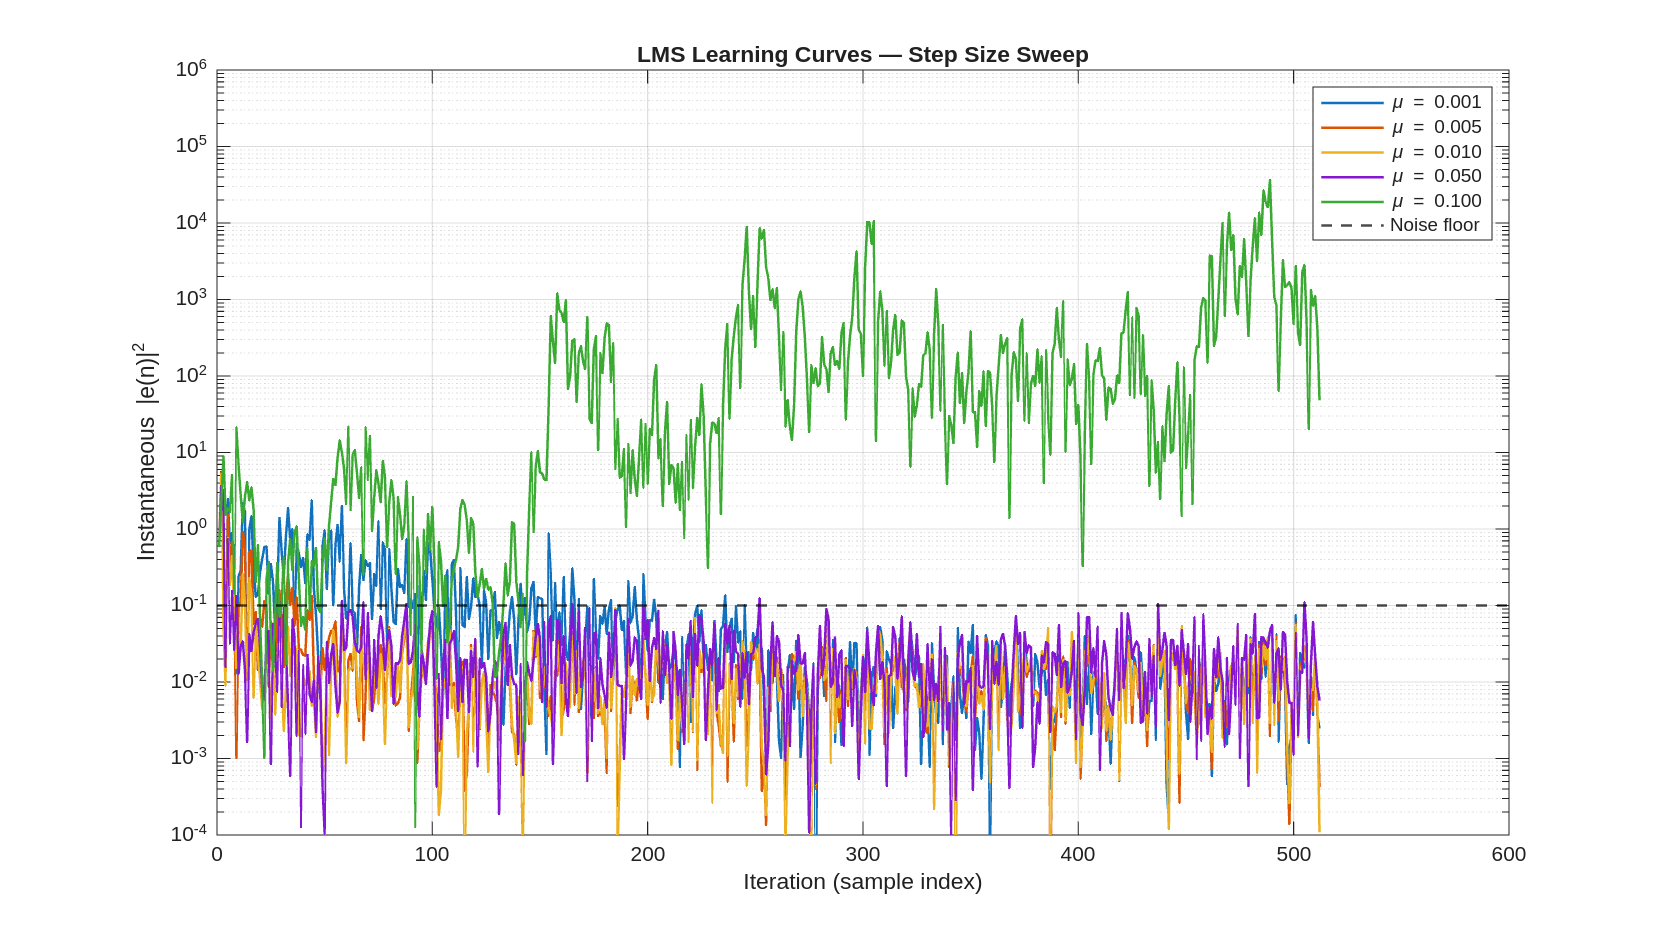
\includegraphics[width=\textwidth]{P2.1_LMS_Learning_Curves.png}
        \caption{Learning curves on log scale. $\mu \leq 0.01$ converge to
                 near the noise floor. $\mu = 0.1$ diverges.}
    \end{subfigure}
    \hfill
    \begin{subfigure}[t]{0.44\textwidth}
        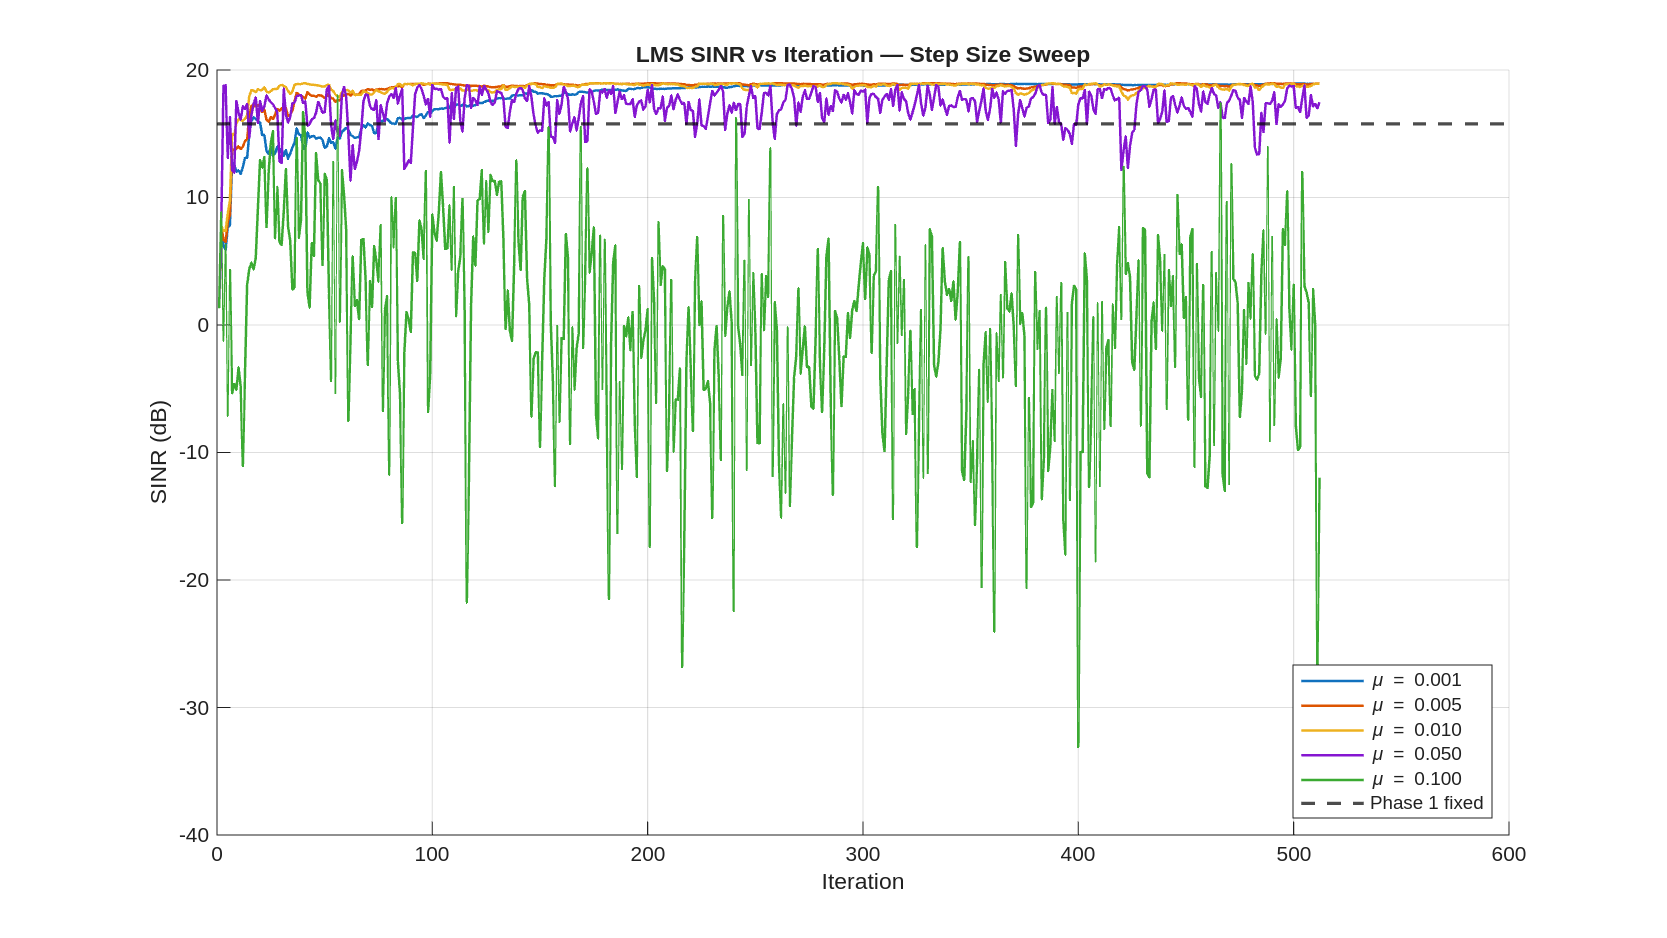
\includegraphics[width=\textwidth]{P2.1_LMS_SINR_Convergence.png}
        \caption{SINR vs iteration. Stable step sizes converge above the
                 Phase~1 fixed-weight baseline (dashed).}
    \end{subfigure}
    \caption{Phase 2.1 --- LMS convergence behaviour.}
\end{figure}

\begin{figure}[H]
    \centering
    \begin{subfigure}[t]{0.54\textwidth}
        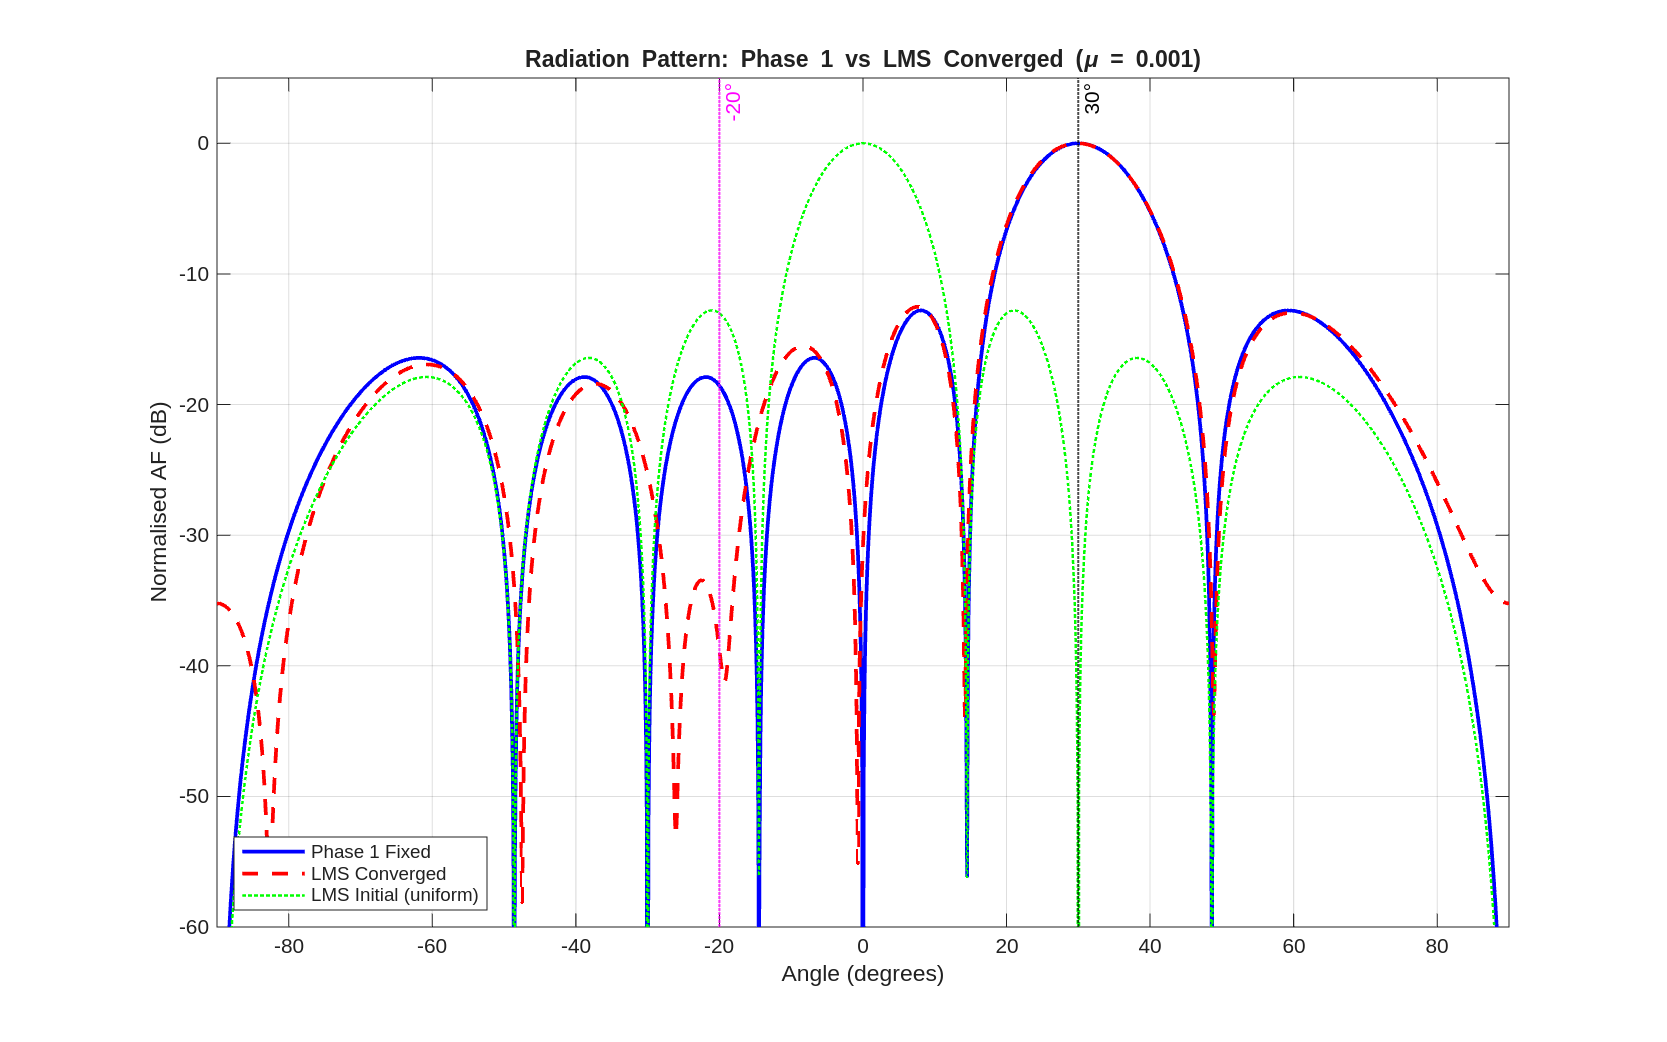
\includegraphics[width=\textwidth]{P2.1_LMS_Pattern_Comparison.png}
        \caption{Radiation pattern: Phase~1 fixed (blue) vs LMS converged
                 (red dashed) vs uniform initial (green dotted). LMS
                 closely matches the Phase~1 pattern.}
    \end{subfigure}
    \hfill
    \begin{subfigure}[t]{0.44\textwidth}
        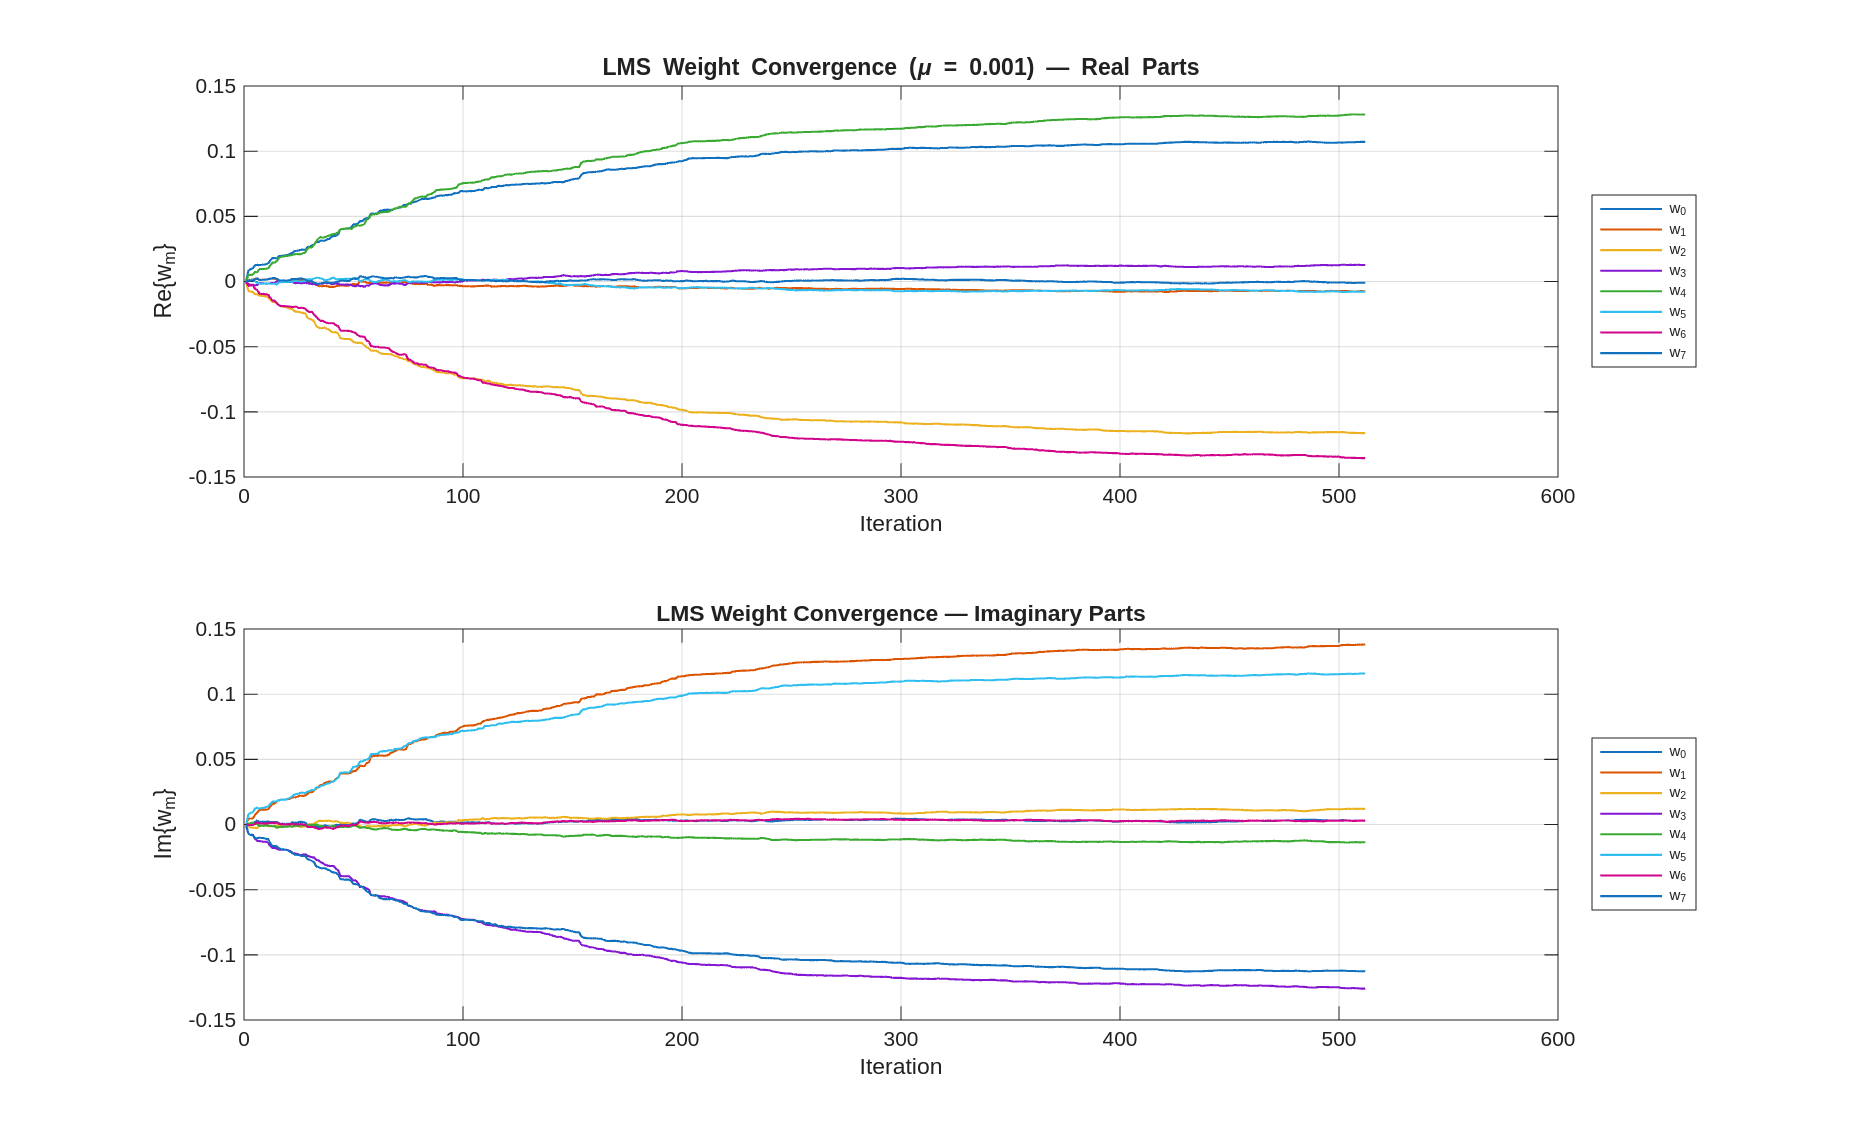
\includegraphics[width=\textwidth]{P2.1_LMS_Weight_Convergence.png}
        \caption{All 8 weight trajectories (real and imaginary parts)
                 from zero to steady state over 512 iterations.}
    \end{subfigure}
    \caption{Phase 2.1 --- LMS converged pattern and weight trajectories.}
\end{figure}

\section{Phase 2.2 --- RLS Adaptive Beamformer Simulation}

The RLS adaptive beamformer was simulated using the same signal environment
as Phases 1.1 and 2.1. The RLS update minimises the exponentially weighted
sum of all past squared errors:
\[
    \mathbf{k}(n) = \frac{\mathbf{P}(n-1)\,\mathbf{x}(n)}
                         {\lambda + \mathbf{x}^H(n)\,\mathbf{P}(n-1)\,\mathbf{x}(n)},
    \quad
    \mathbf{w}(n) = \mathbf{w}(n-1) + \mathbf{k}(n)\,e^*(n),
    \quad
    \mathbf{P}(n) = \frac{1}{\lambda}\left[\mathbf{P}(n-1)
                   - \mathbf{k}(n)\,\mathbf{x}^H(n)\,\mathbf{P}(n-1)\right]
\]

\subsection{Forgetting Factor Sweep}

\begin{table}[H]
\centering
\begin{tabular}{lrl}
\toprule
\textbf{Forgetting factor $\lambda$} & \textbf{Converged SINR} & \textbf{Notes} \\
\midrule
0.900 & +17.17~dB & Fast tracking, higher misadjustment \\
0.950 & +18.26~dB & Moderate \\
0.990 & +18.80~dB & Good balance \\
0.999 & +18.90~dB & Near-optimal \\
1.000 & \textbf{+18.90~dB} & \textcolor{passgreen}{\textbf{Best — stationary channel}} \\
\bottomrule
\end{tabular}
\caption{Phase 2.2 --- RLS forgetting factor sweep results.}
\end{table}

\subsection{Results Summary and Comparison}

\begin{table}[H]
\centering
\begin{tabular}{lrrl}
\toprule
\textbf{Algorithm} & \textbf{Converged SINR} & \textbf{Convergence sample} & \textbf{Complexity} \\
\midrule
Phase~1 Fixed  & +15.78~dB & N/A (no adaptation) & O(1) \\
LMS ($\mu=0.001$) & +18.93~dB & 15 & O($M$) \\
RLS ($\lambda=1.000$) & \textbf{+18.90~dB} & \textbf{2} & O($M^2$) \\
\bottomrule
\end{tabular}
\caption{Phase 2 --- Algorithm comparison summary.}
\end{table}

RLS converges in just \textbf{2 pilot samples} vs LMS's 15, at a cost of
O($M^2$) = O(64) operations per sample vs LMS's O($M$) = O(8). Both
adaptive algorithms exceed the Phase~1 fixed-weight baseline by over 3~dB.
For a stationary channel ($\lambda=1$), RLS is equivalent to a batch
least-squares solution — optimal for the available data.

\begin{figure}[H]
    \centering
    \begin{subfigure}[t]{0.54\textwidth}
        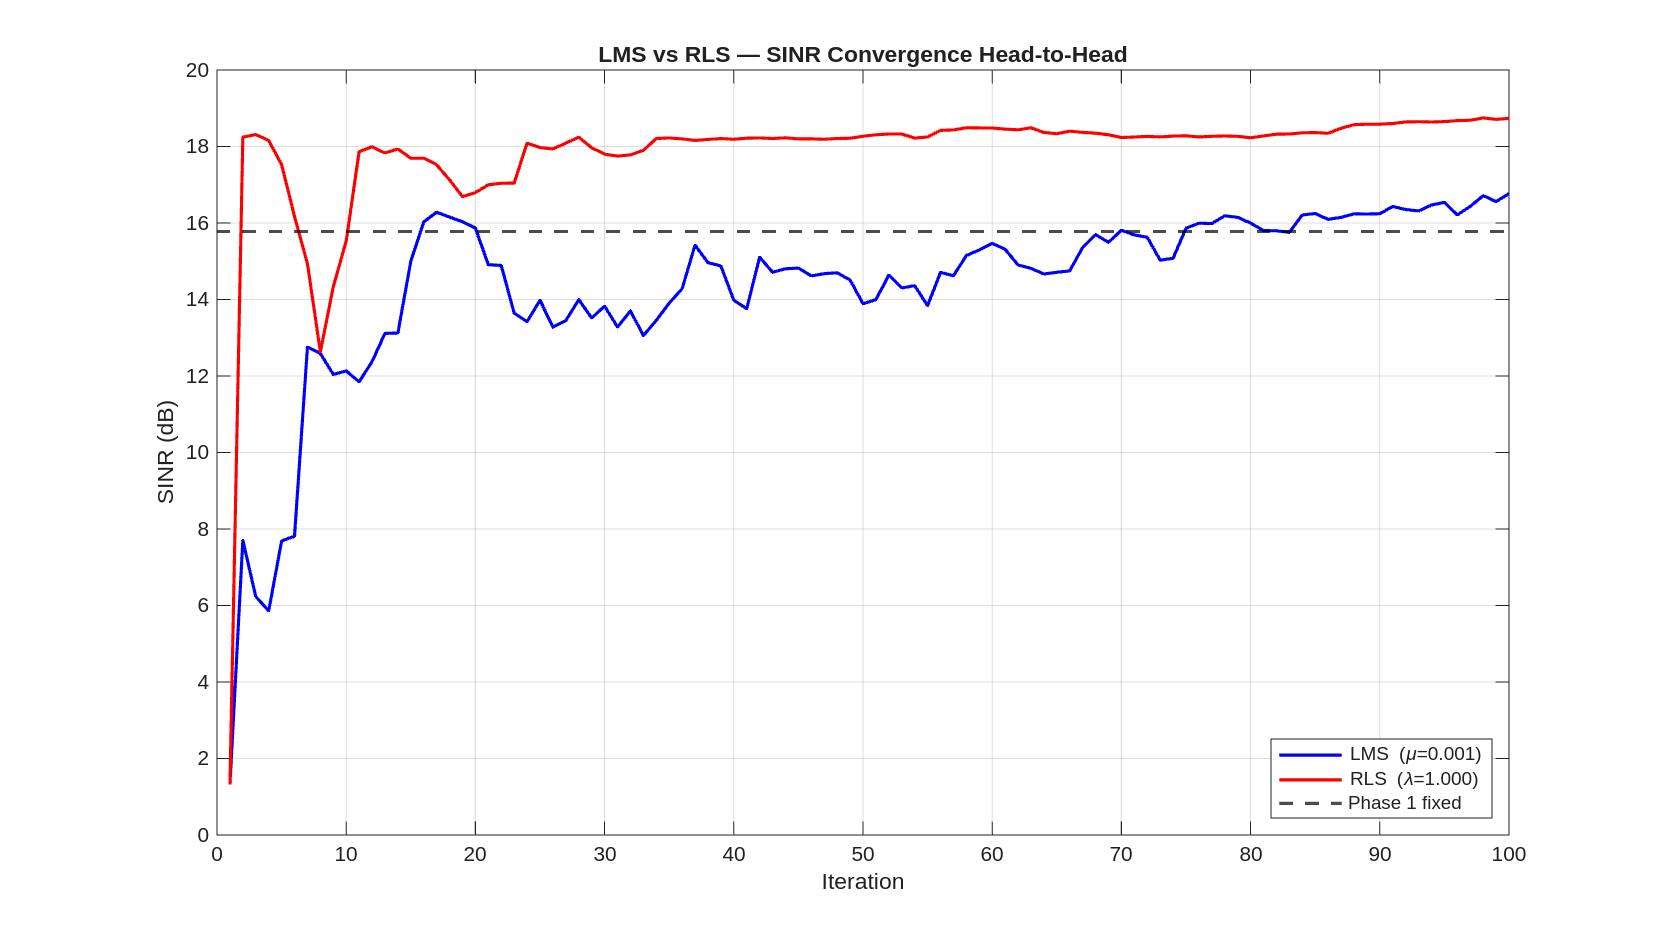
\includegraphics[width=\textwidth]{P2.2_LMS_vs_RLS_Headtohead.png}
        \caption{LMS vs RLS SINR convergence (first 100 samples). RLS
                 exceeds the Phase~1 baseline from sample~2; LMS takes
                 $\sim$80 samples to fully settle.}
    \end{subfigure}
    \hfill
    \begin{subfigure}[t]{0.44\textwidth}
        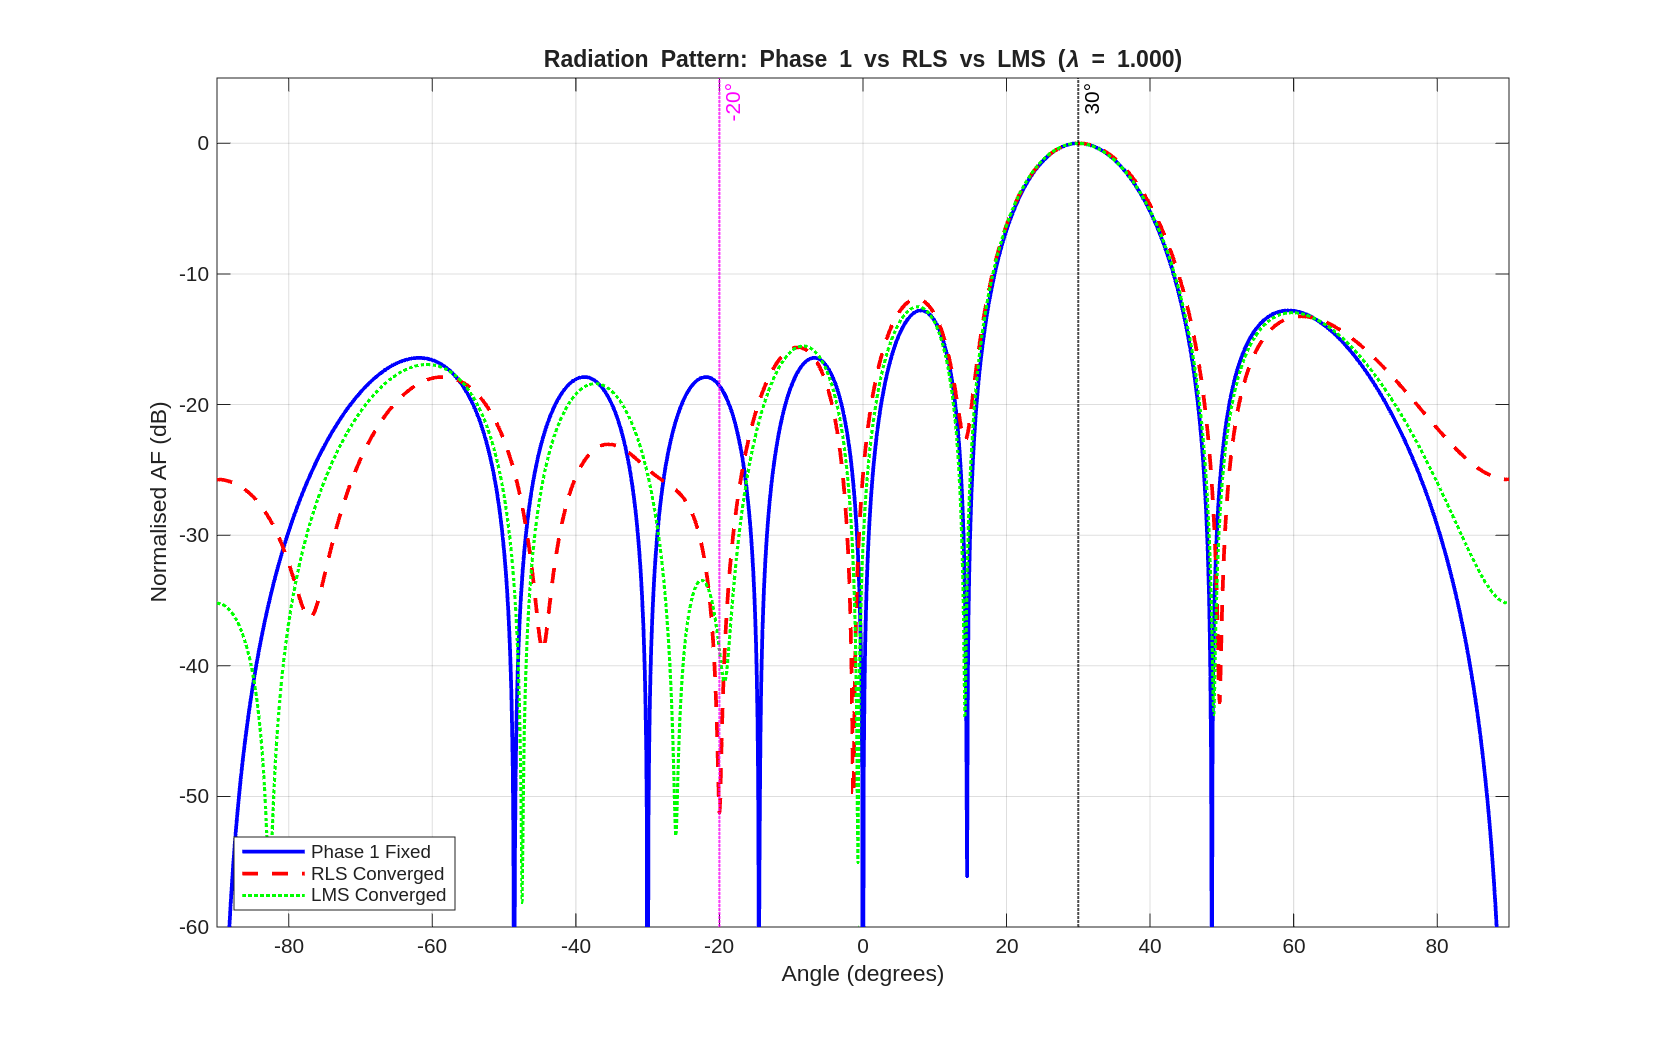
\includegraphics[width=\textwidth]{P2.2_RLS_Pattern_Comparison.png}
        \caption{Radiation patterns: Phase~1 fixed (blue), RLS converged
                 (red dashed), LMS converged (green dotted). All three
                 produce nearly identical beams at 30°.}
    \end{subfigure}
    \caption{Phase 2.2 --- RLS results and head-to-head comparison.}
\end{figure}

\begin{figure}[H]
    \centering
    \begin{subfigure}[t]{0.54\textwidth}
        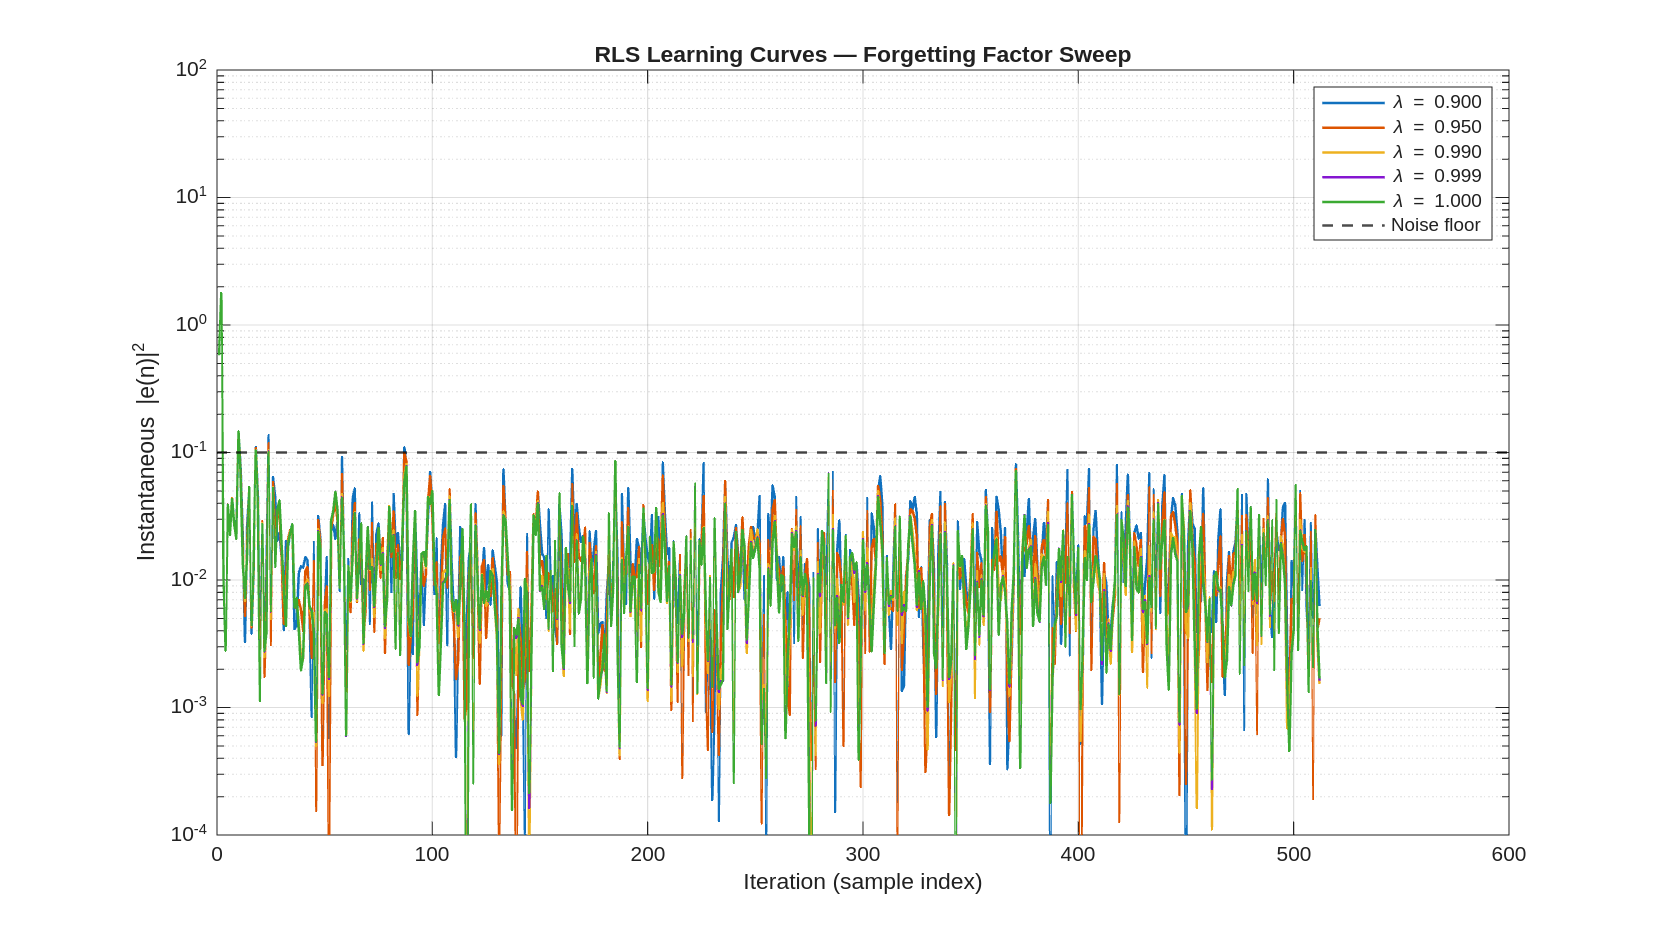
\includegraphics[width=\textwidth]{P2.2_RLS_Learning_Curves.png}
        \caption{RLS learning curves. All forgetting factors converge
                 rapidly; $\lambda < 0.95$ shows higher steady-state
                 error due to excessive down-weighting of past data.}
    \end{subfigure}
    \hfill
    \begin{subfigure}[t]{0.44\textwidth}
        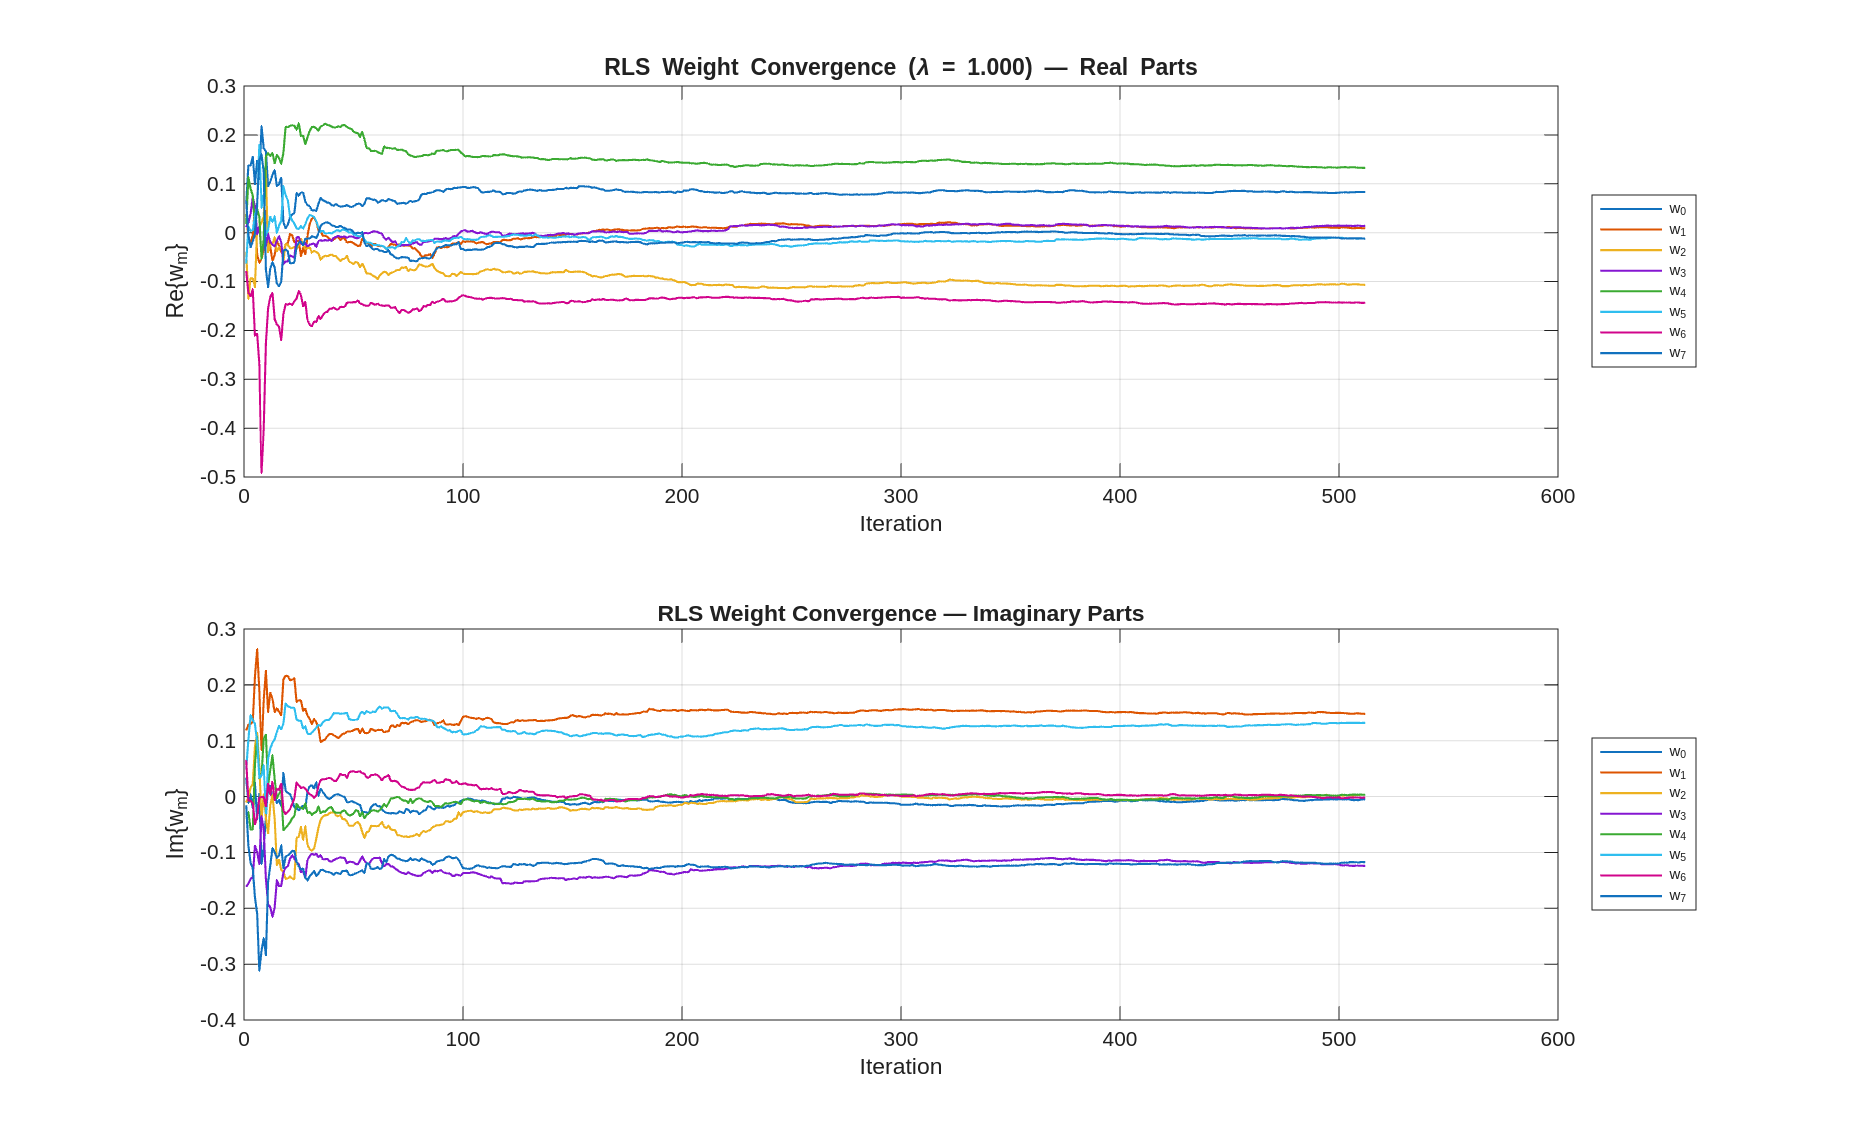
\includegraphics[width=\textwidth]{P2.2_RLS_Weight_Convergence.png}
        \caption{RLS weight trajectories settle within the first
                 $\sim$20 iterations, far faster than LMS.}
    \end{subfigure}
    \caption{Phase 2.2 --- RLS convergence behaviour.}
\end{figure}

\section{Phase 2.3 --- Algorithm Comparison and Recommendation}

\subsection{Consolidated Results}

\begin{table}[H]
\centering
\begin{tabular}{lrrrr}
\toprule
\textbf{Algorithm} & \textbf{SINR} & \textbf{vs Fixed} & \textbf{Conv. sample} & \textbf{MACs/sample} \\
\midrule
Phase~1 Fixed          & +15.78~dB & ---       & N/A & O($M$) = 8 \\
LMS ($\mu$=0.001)      & +18.93~dB & +3.15~dB  & 15  & O($M$) = 32 \\
RLS ($\lambda$=1.000)  & +18.90~dB & +3.12~dB  & 2   & O($M^2$) = 288 \\
\bottomrule
\end{tabular}
\caption{Phase 2.3 --- Final comparison across all three beamformers.}
\end{table}

\subsection{Sensitivity Analysis}

LMS is robust over $\mu \in [0.001,\, 0.010]$ with SINR remaining above
18.8~dB across the stable range. RLS maintains near-peak SINR for
$\lambda \in [0.95,\, 1.000]$; $\lambda < 0.9$ causes excessive
misadjustment. Both algorithms outperform the Phase~1 fixed baseline by
over 3~dB across their respective stable parameter ranges.

\begin{figure}[H]
    \centering
    \begin{subfigure}[t]{0.48\textwidth}
        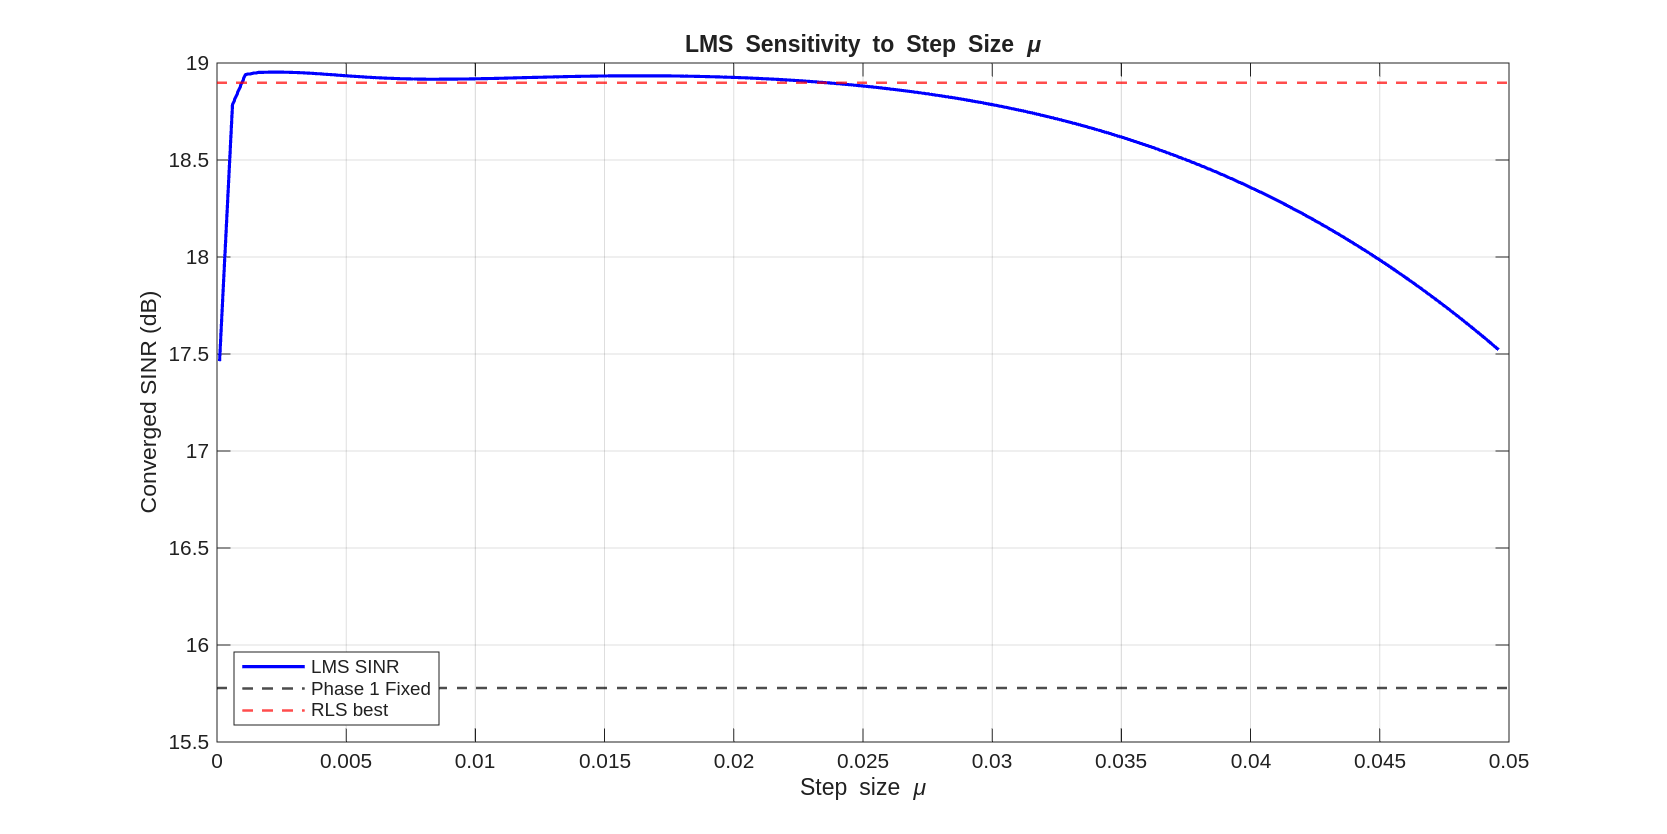
\includegraphics[width=\textwidth]{P2.3_LMS_Sensitivity.png}
        \caption{LMS converged SINR vs step size $\mu$. Flat plateau
                 from $\mu=0.001$ to $0.010$; SINR degrades gracefully
                 above $\mu=0.02$.}
    \end{subfigure}
    \hfill
    \begin{subfigure}[t]{0.48\textwidth}
        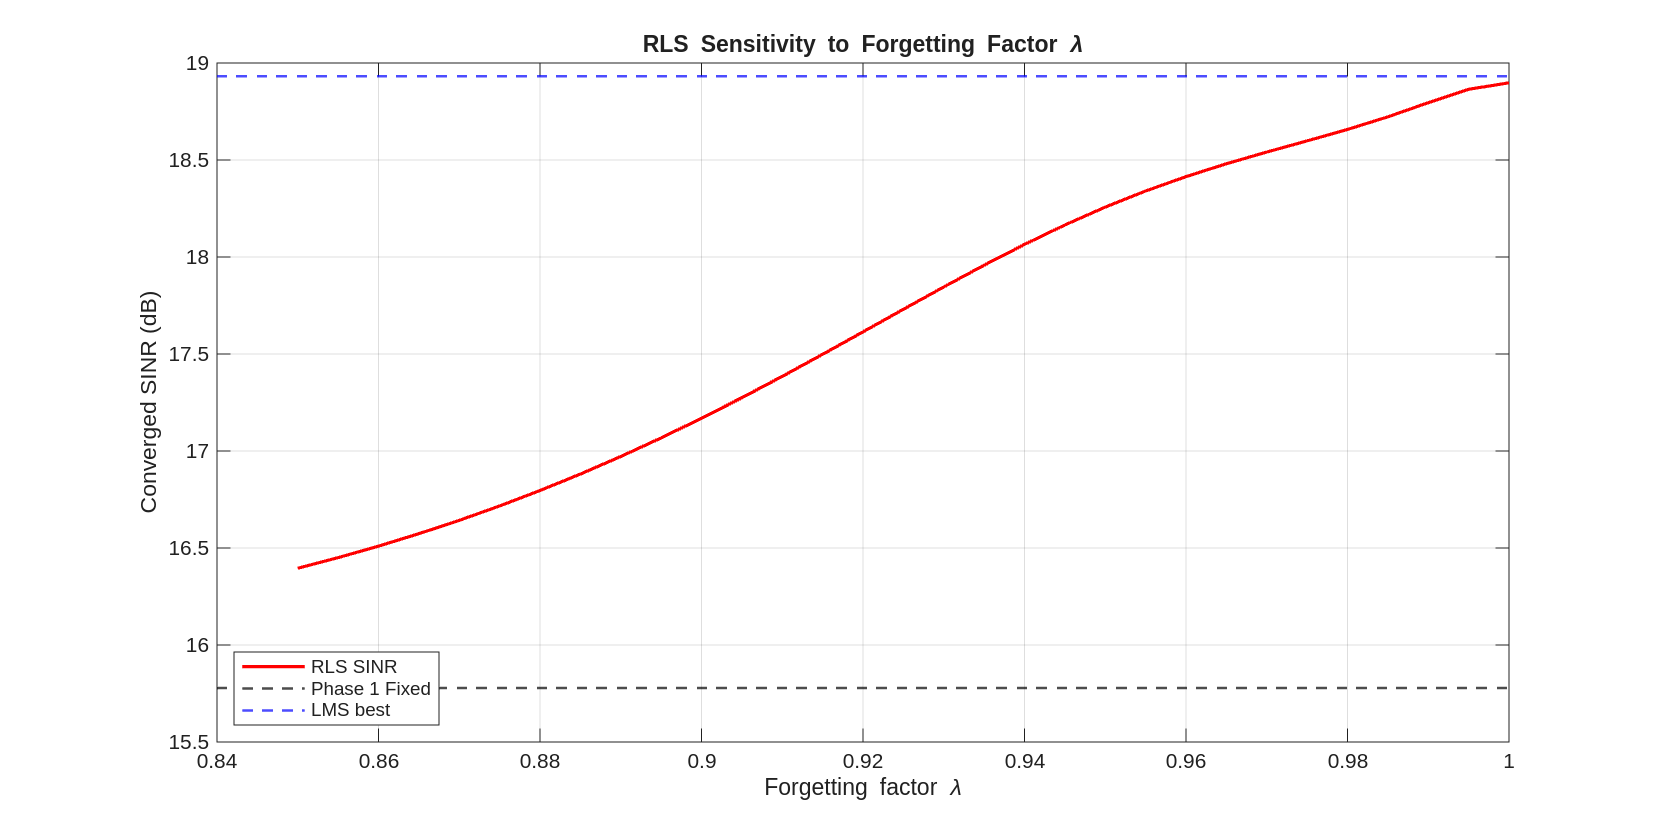
\includegraphics[width=\textwidth]{P2.3_RLS_Sensitivity.png}
        \caption{RLS converged SINR vs forgetting factor $\lambda$.
                 Near-flat for $\lambda \geq 0.97$; drops sharply
                 below $\lambda = 0.92$.}
    \end{subfigure}
    \caption{Phase 2.3 --- Sensitivity of LMS and RLS to parameter choice.}
\end{figure}

\begin{figure}[H]
    \centering
    \begin{subfigure}[t]{0.54\textwidth}
        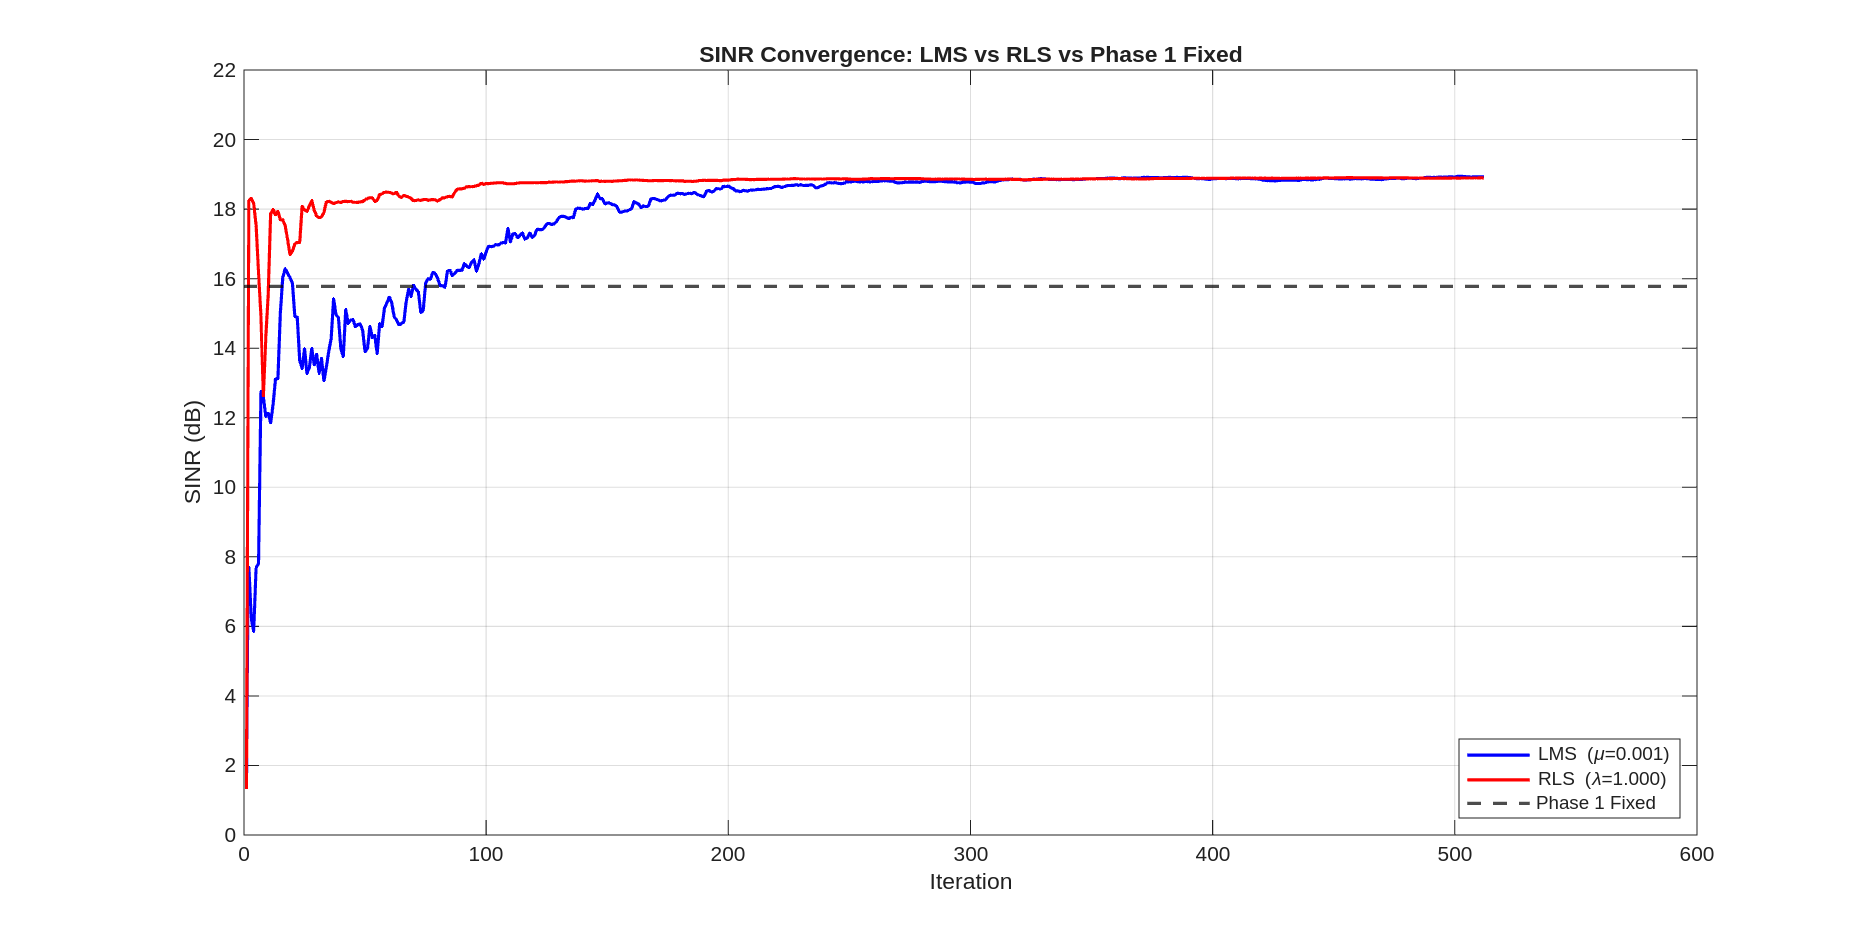
\includegraphics[width=\textwidth]{P2.3_SINR_All_Algorithms.png}
        \caption{Full SINR convergence over 512 samples. RLS (red) leads
                 throughout; LMS (blue) catches up by $\sim$200 samples.
                 Both settle 3~dB above the Phase~1 dashed baseline.}
    \end{subfigure}
    \hfill
    \begin{subfigure}[t]{0.44\textwidth}
        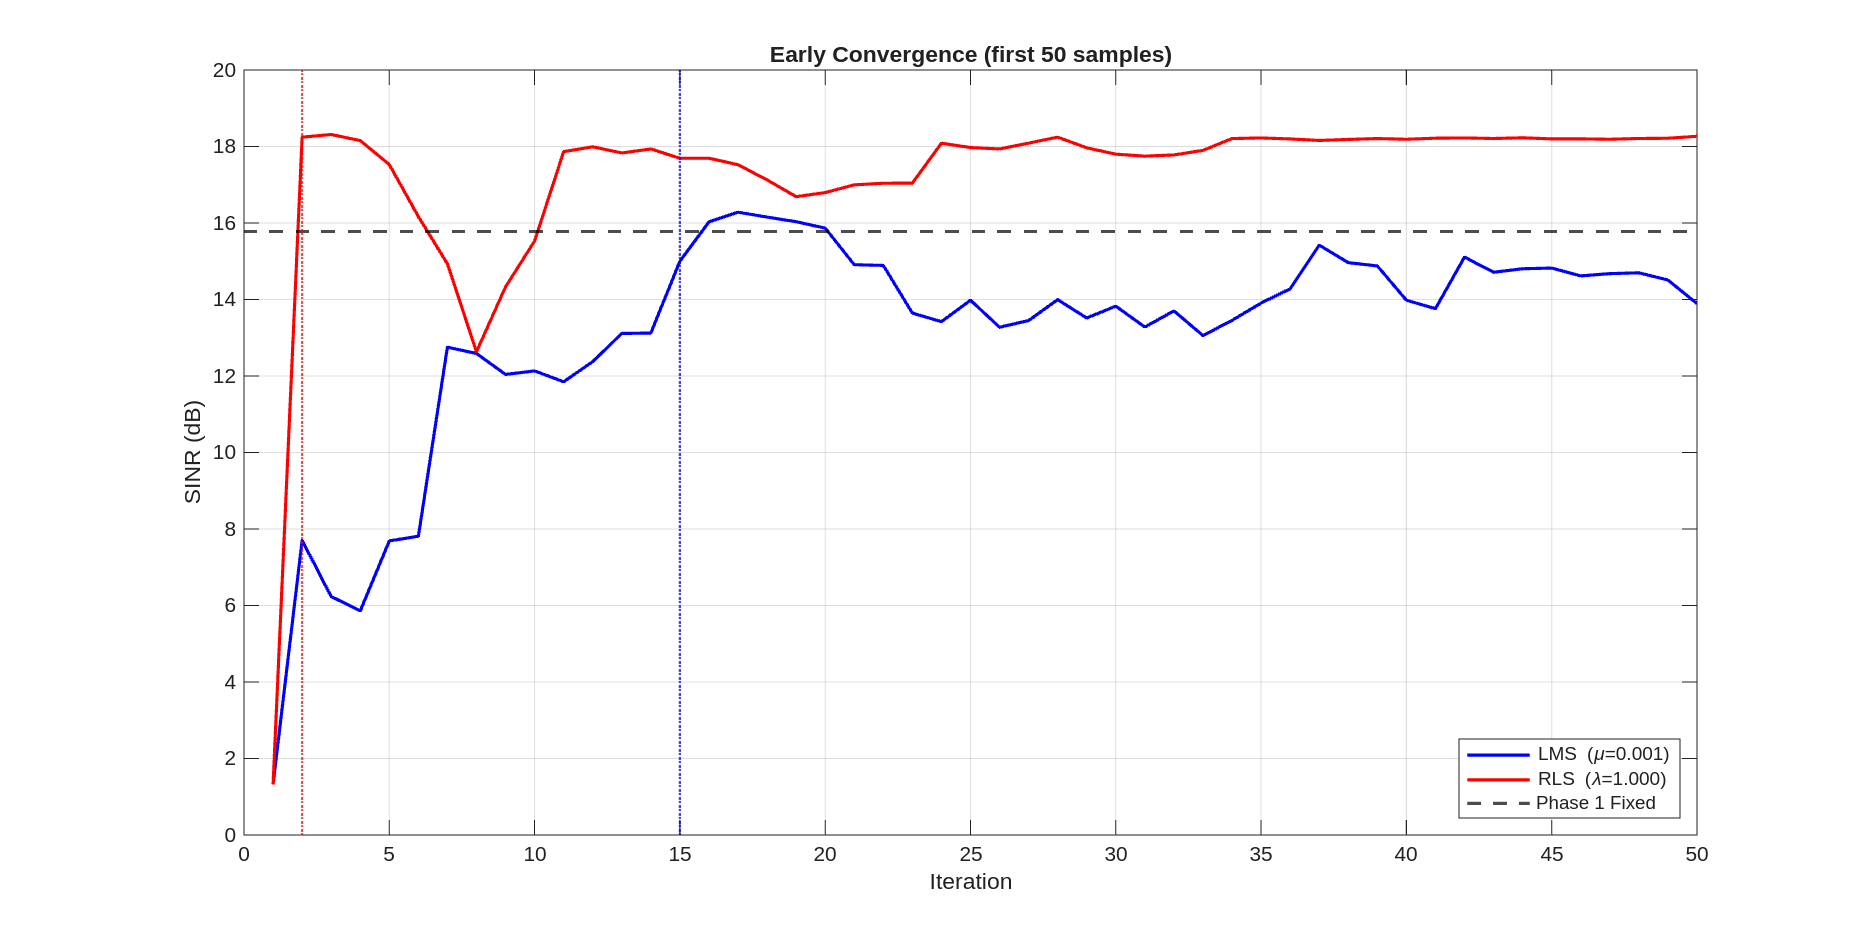
\includegraphics[width=\textwidth]{P2.3_Early_Convergence.png}
        \caption{Zoom on first 50 samples. RLS exceeds the Phase~1
                 baseline at sample~2; LMS crosses it at sample~15.}
    \end{subfigure}
    \caption{Phase 2.3 --- SINR convergence comparison.}
\end{figure}

\begin{figure}[H]
    \centering
    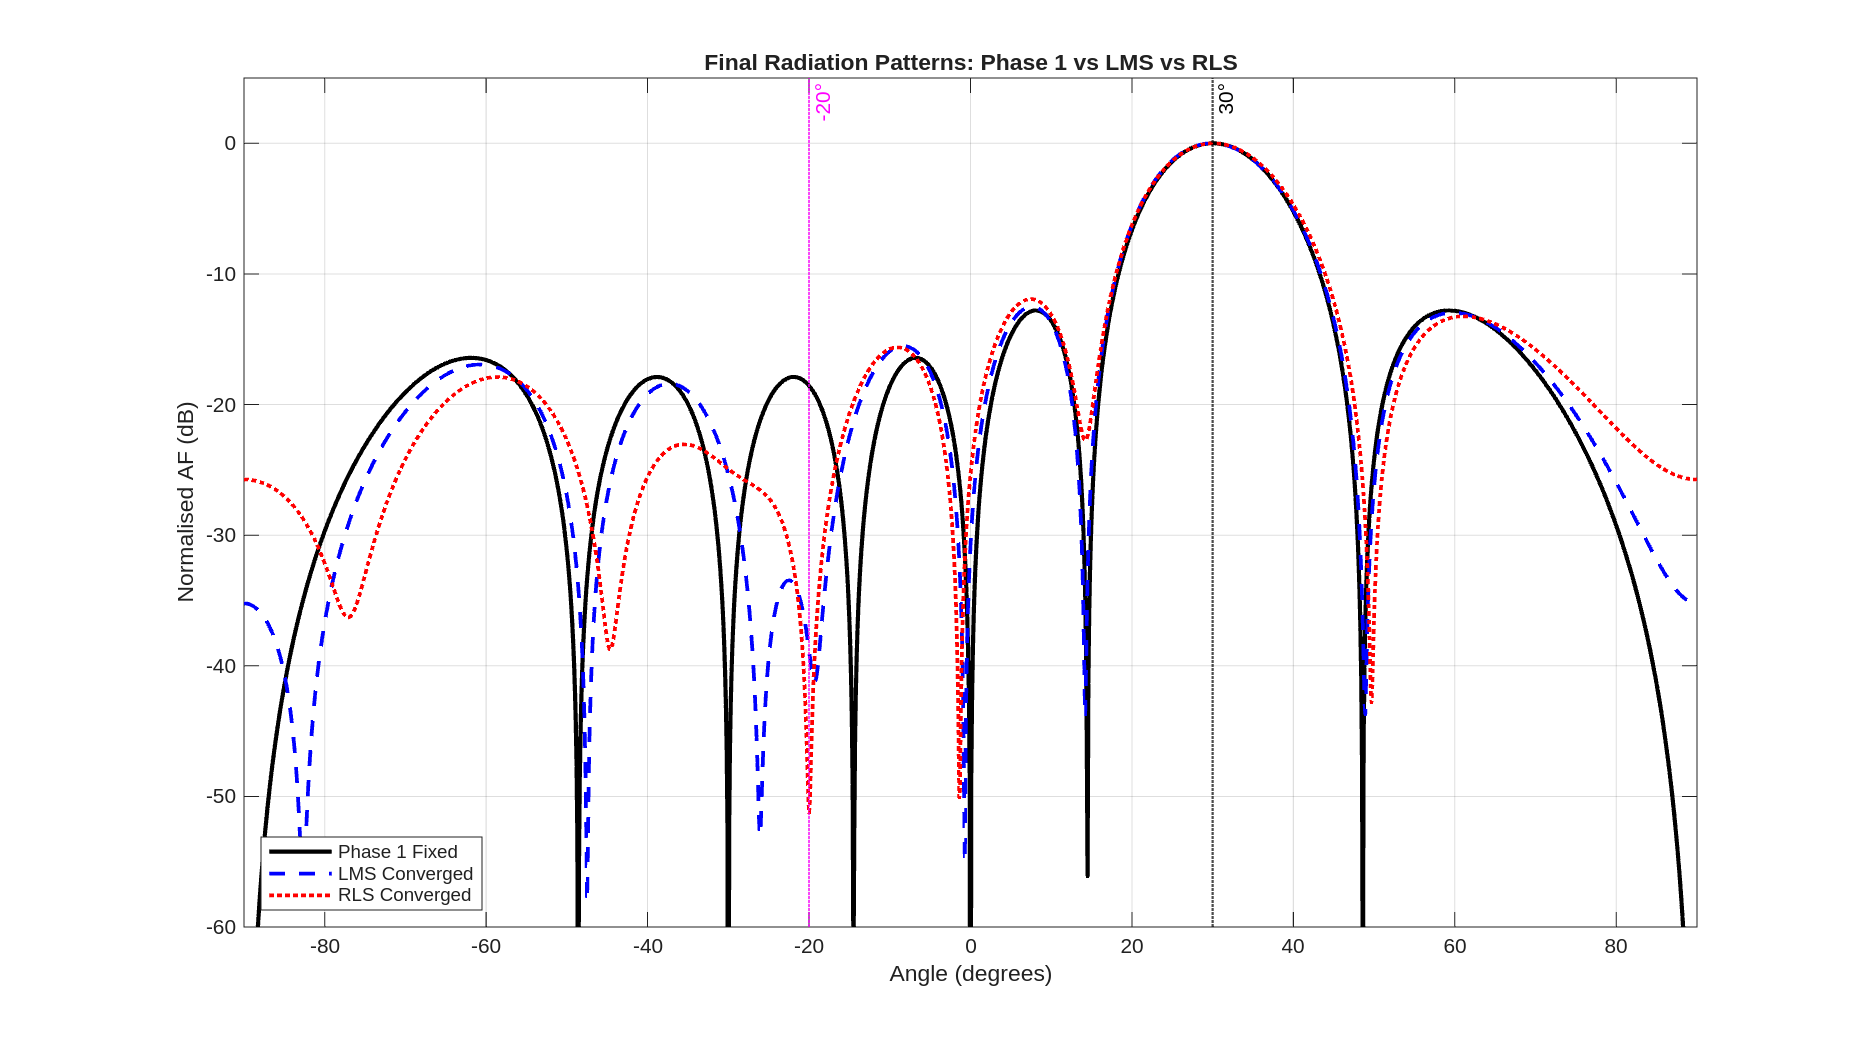
\includegraphics[width=0.65\textwidth]{P2.3_Final_Pattern_All.png}
    \caption{Phase 2.3 --- Final radiation patterns. All three beamformers
             produce a main lobe at 30° with suppression near the
             interferer at $-20°$. LMS and RLS patterns differ slightly
             from Phase~1 in sidelobe structure, reflecting the MSE
             optimisation criterion rather than pure phase steering.}
\end{figure}

\subsection{Recommendation for Future Hardware Implementation}

For a stationary 5G~NR channel with DMRS pilot symbols:

\textbf{Recommended algorithm: LMS with $\mu = 0.001$--$0.005$.}

\begin{itemize}
    \item LMS and RLS achieve near-identical steady-state SINR
          (18.93~dB vs 18.90~dB, $\Delta < 0.03$~dB).
    \item LMS converges in 15 pilot samples --- well within the 5G~NR
          DMRS pilot length of $\sim$100--200 samples per slot.
    \item LMS requires 32~MACs/sample vs RLS's 288~MACs/sample
          (8$\times$ lower hardware cost).
    \item The LMS update maps directly onto the Phase~1 DSP48 pipeline:
          $M$ parallel multiply-accumulate units, same structure as the
          existing data path.
    \item RLS would be preferred for a non-stationary channel
          (fast-moving user) where $\lambda < 1$ is needed for tracking.
          In the static lab scenario simulated here, LMS is sufficient.
\end{itemize}

\vspace{0.5em}\hrule\vspace{0.5em}
{\small\color{neutralgray}
All phases complete. For full design rationale see \texttt{PLAN.md} v3.0.
GitHub: \href{https://github.com/KartikPandeyindia/260410-beamforming}{KartikPandeyindia/260410-beamforming}.}

\vspace{1em}\hrule\vspace{0.5em}
{\small\color{neutralgray}
Generated at end of Phase~1 (Phases 1.1--1.5 complete). Phase~2 direction
revised to MATLAB-only algorithmic study --- see \texttt{PLAN.md} v3.0
for full rationale.
GitHub: \href{https://github.com/KartikPandeyindia/260410-beamforming}{KartikPandeyindia/260410-beamforming}.}

\end{document}
